\documentclass[]{ctexbook}
\usepackage{lmodern}
\usepackage{amssymb,amsmath}
\usepackage{ifxetex,ifluatex}
\usepackage{fixltx2e} % provides \textsubscript
\ifnum 0\ifxetex 1\fi\ifluatex 1\fi=0 % if pdftex
  \usepackage[T1]{fontenc}
  \usepackage[utf8]{inputenc}
\else % if luatex or xelatex
  \ifxetex
    \usepackage{xltxtra,xunicode}
  \else
    \usepackage{fontspec}
  \fi
  \defaultfontfeatures{Ligatures=TeX,Scale=MatchLowercase}
\fi
% use upquote if available, for straight quotes in verbatim environments
\IfFileExists{upquote.sty}{\usepackage{upquote}}{}
% use microtype if available
\IfFileExists{microtype.sty}{%
\usepackage{microtype}
\UseMicrotypeSet[protrusion]{basicmath} % disable protrusion for tt fonts
}{}
\usepackage[b5paper,tmargin=2.5cm,bmargin=2.5cm,lmargin=3.5cm,rmargin=2.5cm]{geometry}
\usepackage[unicode=true]{hyperref}
\PassOptionsToPackage{usenames,dvipsnames}{color} % color is loaded by hyperref
\hypersetup{
            pdftitle={近视预测模型开发与验证},
            pdfauthor={张献伟},
            colorlinks=true,
            linkcolor=Maroon,
            citecolor=Blue,
            urlcolor=Blue,
            breaklinks=true}
\urlstyle{same}  % don't use monospace font for urls
\usepackage{natbib}
\bibliographystyle{apalike}
\usepackage{color}
\usepackage{fancyvrb}
\newcommand{\VerbBar}{|}
\newcommand{\VERB}{\Verb[commandchars=\\\{\}]}
\DefineVerbatimEnvironment{Highlighting}{Verbatim}{commandchars=\\\{\}}
% Add ',fontsize=\small' for more characters per line
\usepackage{framed}
\definecolor{shadecolor}{RGB}{248,248,248}
\newenvironment{Shaded}{\begin{snugshade}}{\end{snugshade}}
\newcommand{\AlertTok}[1]{\textcolor[rgb]{0.94,0.16,0.16}{#1}}
\newcommand{\AnnotationTok}[1]{\textcolor[rgb]{0.56,0.35,0.01}{\textbf{\textit{#1}}}}
\newcommand{\AttributeTok}[1]{\textcolor[rgb]{0.77,0.63,0.00}{#1}}
\newcommand{\BaseNTok}[1]{\textcolor[rgb]{0.00,0.00,0.81}{#1}}
\newcommand{\BuiltInTok}[1]{#1}
\newcommand{\CharTok}[1]{\textcolor[rgb]{0.31,0.60,0.02}{#1}}
\newcommand{\CommentTok}[1]{\textcolor[rgb]{0.56,0.35,0.01}{\textit{#1}}}
\newcommand{\CommentVarTok}[1]{\textcolor[rgb]{0.56,0.35,0.01}{\textbf{\textit{#1}}}}
\newcommand{\ConstantTok}[1]{\textcolor[rgb]{0.00,0.00,0.00}{#1}}
\newcommand{\ControlFlowTok}[1]{\textcolor[rgb]{0.13,0.29,0.53}{\textbf{#1}}}
\newcommand{\DataTypeTok}[1]{\textcolor[rgb]{0.13,0.29,0.53}{#1}}
\newcommand{\DecValTok}[1]{\textcolor[rgb]{0.00,0.00,0.81}{#1}}
\newcommand{\DocumentationTok}[1]{\textcolor[rgb]{0.56,0.35,0.01}{\textbf{\textit{#1}}}}
\newcommand{\ErrorTok}[1]{\textcolor[rgb]{0.64,0.00,0.00}{\textbf{#1}}}
\newcommand{\ExtensionTok}[1]{#1}
\newcommand{\FloatTok}[1]{\textcolor[rgb]{0.00,0.00,0.81}{#1}}
\newcommand{\FunctionTok}[1]{\textcolor[rgb]{0.00,0.00,0.00}{#1}}
\newcommand{\ImportTok}[1]{#1}
\newcommand{\InformationTok}[1]{\textcolor[rgb]{0.56,0.35,0.01}{\textbf{\textit{#1}}}}
\newcommand{\KeywordTok}[1]{\textcolor[rgb]{0.13,0.29,0.53}{\textbf{#1}}}
\newcommand{\NormalTok}[1]{#1}
\newcommand{\OperatorTok}[1]{\textcolor[rgb]{0.81,0.36,0.00}{\textbf{#1}}}
\newcommand{\OtherTok}[1]{\textcolor[rgb]{0.56,0.35,0.01}{#1}}
\newcommand{\PreprocessorTok}[1]{\textcolor[rgb]{0.56,0.35,0.01}{\textit{#1}}}
\newcommand{\RegionMarkerTok}[1]{#1}
\newcommand{\SpecialCharTok}[1]{\textcolor[rgb]{0.00,0.00,0.00}{#1}}
\newcommand{\SpecialStringTok}[1]{\textcolor[rgb]{0.31,0.60,0.02}{#1}}
\newcommand{\StringTok}[1]{\textcolor[rgb]{0.31,0.60,0.02}{#1}}
\newcommand{\VariableTok}[1]{\textcolor[rgb]{0.00,0.00,0.00}{#1}}
\newcommand{\VerbatimStringTok}[1]{\textcolor[rgb]{0.31,0.60,0.02}{#1}}
\newcommand{\WarningTok}[1]{\textcolor[rgb]{0.56,0.35,0.01}{\textbf{\textit{#1}}}}
\usepackage{longtable,booktabs}
% Fix footnotes in tables (requires footnote package)
\IfFileExists{footnote.sty}{\usepackage{footnote}\makesavenoteenv{long table}}{}
\usepackage{graphicx,grffile}
\makeatletter
\def\maxwidth{\ifdim\Gin@nat@width>\linewidth\linewidth\else\Gin@nat@width\fi}
\def\maxheight{\ifdim\Gin@nat@height>\textheight\textheight\else\Gin@nat@height\fi}
\makeatother
% Scale images if necessary, so that they will not overflow the page
% margins by default, and it is still possible to overwrite the defaults
% using explicit options in \includegraphics[width, height, ...]{}
\setkeys{Gin}{width=\maxwidth,height=\maxheight,keepaspectratio}
\IfFileExists{parskip.sty}{%
\usepackage{parskip}
}{% else
\setlength{\parindent}{0pt}
\setlength{\parskip}{6pt plus 2pt minus 1pt}
}
\setlength{\emergencystretch}{3em}  % prevent overfull lines
\providecommand{\tightlist}{%
  \setlength{\itemsep}{0pt}\setlength{\parskip}{0pt}}
\setcounter{secnumdepth}{5}
% Redefines (sub)paragraphs to behave more like sections
\ifx\paragraph\undefined\else
\let\oldparagraph\paragraph
\renewcommand{\paragraph}[1]{\oldparagraph{#1}\mbox{}}
\fi
\ifx\subparagraph\undefined\else
\let\oldsubparagraph\subparagraph
\renewcommand{\subparagraph}[1]{\oldsubparagraph{#1}\mbox{}}
\fi

% set default figure placement to htbp
\makeatletter
\def\fps@figure{htbp}
\makeatother

\usepackage{booktabs}
\usepackage{longtable}

\usepackage{framed,color}
\definecolor{shadecolor}{RGB}{248,248,248}

\renewcommand{\textfraction}{0.05}
\renewcommand{\topfraction}{0.8}
\renewcommand{\bottomfraction}{0.8}
\renewcommand{\floatpagefraction}{0.75}

\let\oldhref\href
\renewcommand{\href}[2]{#2\footnote{\url{#1}}}

\makeatletter
\newenvironment{kframe}{%
\medskip{}
\setlength{\fboxsep}{.8em}
 \def\at@end@of@kframe{}%
 \ifinner\ifhmode%
  \def\at@end@of@kframe{\end{minipage}}%
  \begin{minipage}{\columnwidth}%
 \fi\fi%
 \def\FrameCommand##1{\hskip\@totalleftmargin \hskip-\fboxsep
 \colorbox{shadecolor}{##1}\hskip-\fboxsep
     % There is no \\@totalrightmargin, so:
     \hskip-\linewidth \hskip-\@totalleftmargin \hskip\columnwidth}%
 \MakeFramed {\advance\hsize-\width
   \@totalleftmargin\z@ \linewidth\hsize
   \@setminipage}}%
 {\par\unskip\endMakeFramed%
 \at@end@of@kframe}
\makeatother

\makeatletter
\@ifundefined{Shaded}{
}{\renewenvironment{Shaded}{\begin{kframe}}{\end{kframe}}}
\@ifpackageloaded{fancyvrb}{%
  % https://github.com/CTeX-org/ctex-kit/issues/331
  \RecustomVerbatimEnvironment{Highlighting}{Verbatim}{commandchars=\\\{\},formatcom=\xeCJKVerbAddon}%
}{}
\makeatother

\usepackage{makeidx}
\makeindex

\urlstyle{tt}

\usepackage{amsthm}
\makeatletter
\def\thm@space@setup{%
  \thm@preskip=8pt plus 2pt minus 4pt
  \thm@postskip=\thm@preskip
}
\makeatother

\frontmatter

\title{近视预测模型开发与验证}
\author{张献伟}
\date{2022-07-25}

\begin{document}
\maketitle


\thispagestyle{empty}

\begin{center}
献给……

呃,爱谁谁吧
\end{center}

\setlength{\abovedisplayskip}{-5pt}
\setlength{\abovedisplayshortskip}{-5pt}

{
\setcounter{tocdepth}{2}
\tableofcontents
}
\listoftables
\listoffigures
\hypertarget{ux524dux8a00}{%
\chapter*{前言}\label{ux524dux8a00}}


你好,世界。我写了一本书。这本书是这样的,第 \ref{intro} 章介绍了见第\ref{intro},第 \ref{wind} 章说见\ref{wind},然后是请自己阅读吧!!!

我用了两个 R 包编译这本书,分别是 \textbf{knitr}\index{knitr} \citep{xie2015} 和 \textbf{bookdown}\index{bookdown} \citep{R-bookdown}。以下是我的 R 进程信息:

\begin{Shaded}
\begin{Highlighting}[]
\FunctionTok{sessionInfo}\NormalTok{()}
\end{Highlighting}
\end{Shaded}

\begin{verbatim}
## R version 4.1.1 (2021-08-10)
## Platform: x86_64-w64-mingw32/x64 (64-bit)
## Running under: Windows 7 x64 (build 7601) Service Pack 1
## 
## Matrix products: default
## 
## locale:
## [1] LC_COLLATE=Chinese (Simplified)_People's Republic of China.936 
## [2] LC_CTYPE=Chinese (Simplified)_People's Republic of China.936   
## [3] LC_MONETARY=Chinese (Simplified)_People's Republic of China.936
## [4] LC_NUMERIC=C                                                   
## [5] LC_TIME=Chinese (Simplified)_People's Republic of China.936    
## 
## attached base packages:
## [1] stats     graphics  grDevices utils     datasets 
## [6] methods   base     
## 
## loaded via a namespace (and not attached):
##  [1] compiler_4.1.1  magrittr_2.0.1  fastmap_1.1.0  
##  [4] bookdown_0.24   cli_3.3.0       htmltools_0.5.2
##  [7] tools_4.1.1     rstudioapi_0.13 yaml_2.2.1     
## [10] stringi_1.7.4   rmarkdown_2.11  knitr_1.34     
## [13] stringr_1.4.0   digest_0.6.27   xfun_0.25      
## [16] rlang_1.0.4     evaluate_0.14
\end{verbatim}

\hypertarget{ux81f4ux8c22}{%
\section*{致谢}\label{ux81f4ux8c22}}


感谢我自己的努力。

\begin{flushright}
张献伟\\
于 某角落
\end{flushright}

\hypertarget{author}{%
\chapter*{作者简介}\label{author}}


尘世中一个迷途小书童

\mainmatter

\hypertarget{ux4e34ux5e8aux9884ux6d4bux6a21ux578b}{%
\chapter{临床预测模型}\label{ux4e34ux5e8aux9884ux6d4bux6a21ux578b}}

常见的思路总结为三步:

1.模型构建

2.模型评价

3.模型验证

\hypertarget{ux6a21ux578bux6784ux5efa}{%
\section{模型构建}\label{ux6a21ux578bux6784ux5efa}}

最熟悉的方法是:先单后多。大多数可行。但当变量数过多,变量之间存在共线性或缺失值过多而又不愿舍弃掉缺失值的样本, 有局限性。

如何解决?

1.共线性问题------岭回归、\emph{lasso}、弹性网络模型(正则技术)

2.缺失值问题------随机森林模型

要解决的主要问题:变量筛选

方法1:逐步回归(向后法、向前法、向前向后法)

方法2:正则技术(岭回归、lasso、弹性网络模型)

方法3:树模型

方法4:随机森林模型(树模型的扩展)

方法5:主成分分析

\hypertarget{ux6a21ux578bux8bc4ux4ef7}{%
\section{模型评价}\label{ux6a21ux578bux8bc4ux4ef7}}

为什么要评价模型?

\begin{itemize}
\tightlist
\item
  欠拟合
\item
  过拟合
\end{itemize}

常见的评价指标主要有以下几种
1.拟合优度检验(涉及卡方值及P值)

2.ROC(涉及AUC,sen,spe,accuracy等指标)

3.calibration(涉及C-index的计算)

4.终极指标MSE的计算

5.其他

通常来说,完成模型评价已经可以称之为''完整''的研究。

\textbf{过拟合呢?或者是外推性如何?}

\hypertarget{ux6a21ux578bux9a8cux8bc1}{%
\section{模型验证}\label{ux6a21ux578bux9a8cux8bc1}}

1.cross validation(\emph{简单交叉};K-fold corss validation;N-fold cross validation)
2.bootstrap
3.crossvalidation+bootstrap(最常用)

ps:三个过程可能需要多次操作,才可以得到最终的结果。

\hypertarget{ux6570ux636e}{%
\chapter{数据}\label{ux6570ux636e}}

\hypertarget{ux6570ux636eux96c6ux7b80ux4ecb}{%
\section{数据集简介}\label{ux6570ux636eux96c6ux7b80ux4ecb}}

该数据集是来自 Orinda 近视纵向研究 (OLSM) 的数据子集,这是一项眼科队列研究儿童近视发病的成分发育和危险因素。 数据收集始于 1989-1990 年学年,并每年持续到 2000-2001 学年。 有关构成眼睛的部分的所有数据(眼部成分)是在上学期间的一次考试中收集的。 家族史数据和在家长或监护人完成的一项调查中,每年都会收集视觉活动。

本文中使用的数据集来自 618 名至少接受五年随访且非近视的受试者
当他们进入队列时, 所有数据都来自他们的初始检查,数据集包括 17 个变量。 此外眼睛数据有关于进入年龄,进入年份,近视家族史和各种视觉小时数的信息活动。 眼部数据来自受试者的右眼。

\begin{Shaded}
\begin{Highlighting}[]
\NormalTok{data }\OtherTok{\textless{}{-}} \FunctionTok{read.csv}\NormalTok{(}\StringTok{\textquotesingle{}myopia.csv\textquotesingle{}}\NormalTok{)}
\FunctionTok{library}\NormalTok{(knitr)}
\NormalTok{knitr}\SpecialCharTok{::}\FunctionTok{kable}\NormalTok{(}\FunctionTok{head}\NormalTok{(data)) }
\end{Highlighting}
\end{Shaded}

\begin{tabular}{r|r|r|r|r|r|r|r|r|r|r|r|r|r|r|r|r|r}
\hline
ID & STUDYYEAR & MYOPIC & AGE & GENDER & SPHEQ & AL & ACD & LT & VCD & SPORTHR & READHR & COMPHR & STUDYHR & TVHR & DIOPTERHR & MOMMY & DADMY\\
\hline
1 & 1992 & 1 & 6 & 1 & -0.052 & 21.89 & 3.690 & 3.498 & 14.70 & 45 & 8 & 0 & 0 & 10 & 34 & 1 & 1\\
\hline
2 & 1995 & 0 & 6 & 1 & 0.608 & 22.38 & 3.702 & 3.392 & 15.29 & 4 & 0 & 1 & 1 & 7 & 12 & 1 & 1\\
\hline
3 & 1991 & 0 & 6 & 1 & 1.179 & 22.49 & 3.462 & 3.514 & 15.52 & 14 & 0 & 2 & 0 & 10 & 14 & 0 & 0\\
\hline
4 & 1990 & 1 & 6 & 1 & 0.525 & 22.20 & 3.862 & 3.612 & 14.73 & 18 & 11 & 0 & 0 & 4 & 37 & 0 & 1\\
\hline
5 & 1995 & 0 & 5 & 0 & 0.697 & 23.29 & 3.676 & 3.454 & 16.16 & 14 & 0 & 0 & 0 & 4 & 4 & 1 & 0\\
\hline
6 & 1995 & 0 & 6 & 0 & 1.744 & 22.14 & 3.224 & 3.556 & 15.36 & 10 & 6 & 2 & 1 & 19 & 44 & 0 & 1\\
\hline
\end{tabular}

\hypertarget{ux7528sphequx9884ux6d4bux8fd1ux89c6}{%
\section{用SPHEQ预测近视}\label{ux7528sphequx9884ux6d4bux8fd1ux89c6}}

\begin{Shaded}
\begin{Highlighting}[]
\FunctionTok{library}\NormalTok{(tidyverse)}
\end{Highlighting}
\end{Shaded}

\begin{verbatim}
## Warning: replacing previous import 'lifecycle::last_warnings' by
## 'rlang::last_warnings' when loading 'pillar'
\end{verbatim}

\begin{verbatim}
## Warning: replacing previous import 'lifecycle::last_warnings' by
## 'rlang::last_warnings' when loading 'hms'
\end{verbatim}

\begin{verbatim}
## -- Attaching packages --------------------------------------- tidyverse 1.3.1 --
\end{verbatim}

\begin{verbatim}
## v ggplot2 3.3.5     v purrr   0.3.4
## v tibble  3.1.7     v dplyr   1.0.7
## v tidyr   1.1.3     v stringr 1.4.0
## v readr   2.0.1     v forcats 0.5.1
\end{verbatim}

\begin{verbatim}
## Warning: 程辑包'tibble'是用R版本4.1.3 来建造的
\end{verbatim}

\begin{verbatim}
## -- Conflicts ------------------------------------------ tidyverse_conflicts() --
## x dplyr::filter() masks stats::filter()
## x dplyr::lag()    masks stats::lag()
\end{verbatim}

\begin{Shaded}
\begin{Highlighting}[]
\NormalTok{data }\SpecialCharTok{\%\textgreater{}\%} 
  \FunctionTok{ggplot}\NormalTok{(.,}\FunctionTok{aes}\NormalTok{(}\AttributeTok{x=}\NormalTok{SPHEQ,}\AttributeTok{y=}\NormalTok{MYOPIC))}\SpecialCharTok{+}
  \FunctionTok{geom\_jitter}\NormalTok{(}\AttributeTok{shape=}\StringTok{"O"}\NormalTok{,}\AttributeTok{position =} \FunctionTok{position\_jitter}\NormalTok{(}\AttributeTok{height =} \DecValTok{0}\NormalTok{))}\SpecialCharTok{+}
  \FunctionTok{theme\_bw}\NormalTok{()}
\end{Highlighting}
\end{Shaded}

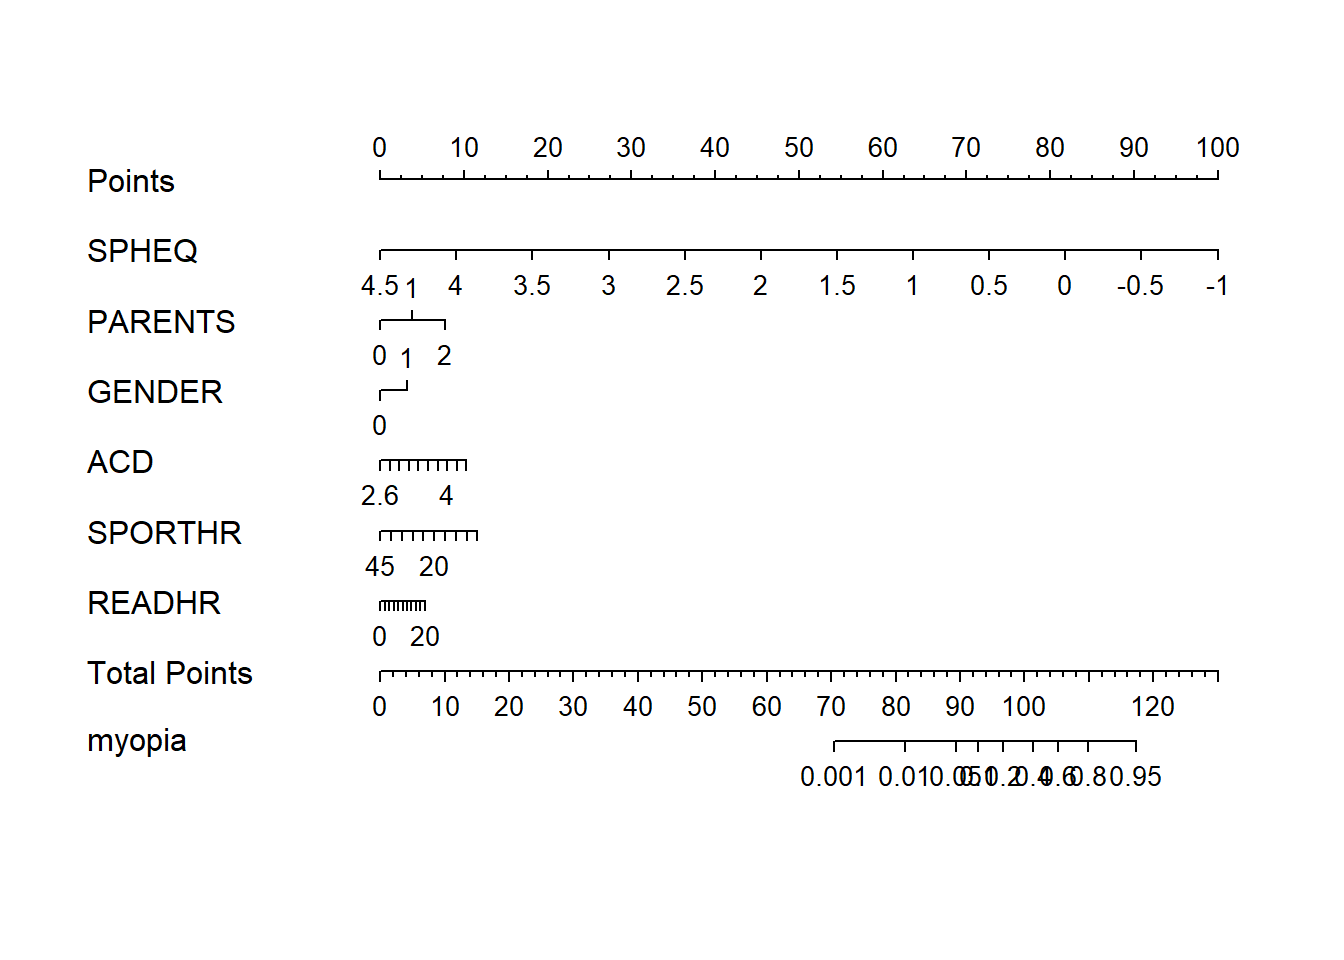
\includegraphics{02-foo_files/figure-latex/unnamed-chunk-2-1.pdf}

在这种情况下,``SPHEQ''显然会影响近视的存在,但不足以准确预测。 需要向模型添加更多属性以改进
预测。 为此,需要检查每个属性与近视存在之间的相关性。

\hypertarget{ux7ed8ux5236ux6240ux6709ux53d8ux91cfux4e4bux95f4ux7684ux76f8ux5173ux6027}{%
\section{绘制所有变量之间的相关性}\label{ux7ed8ux5236ux6240ux6709ux53d8ux91cfux4e4bux95f4ux7684ux76f8ux5173ux6027}}

\begin{Shaded}
\begin{Highlighting}[]
\FunctionTok{library}\NormalTok{(corrplot)}
\end{Highlighting}
\end{Shaded}

\begin{verbatim}
## Warning: 程辑包'corrplot'是用R版本4.1.2 来建造的
\end{verbatim}

\begin{verbatim}
## corrplot 0.92 loaded
\end{verbatim}

\begin{Shaded}
\begin{Highlighting}[]
\FunctionTok{corrplot.mixed}\NormalTok{(}\FunctionTok{cor}\NormalTok{(data))}
\end{Highlighting}
\end{Shaded}

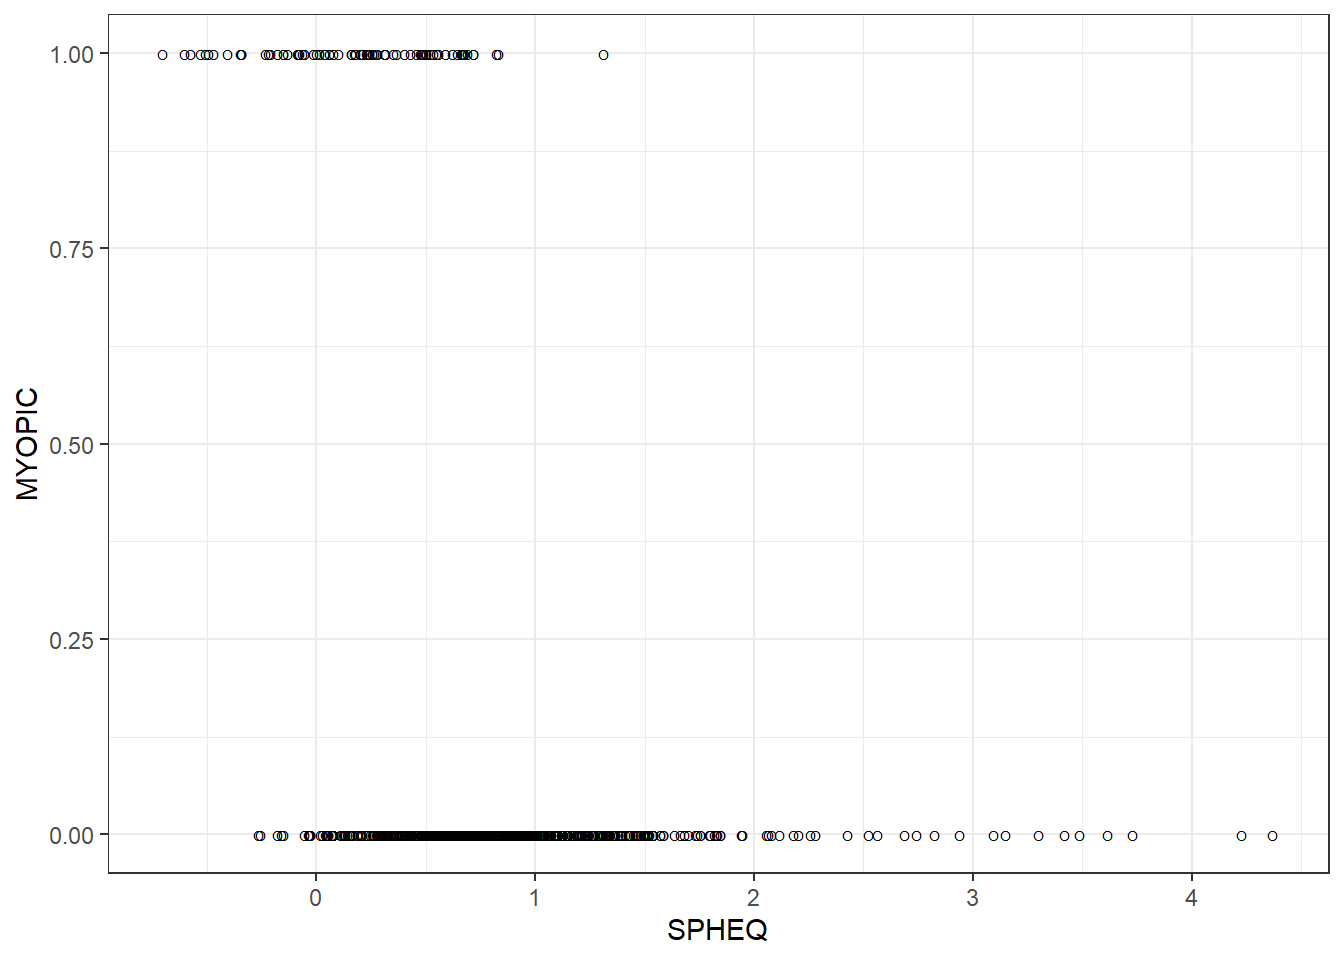
\includegraphics{02-foo_files/figure-latex/unnamed-chunk-3-1.pdf}

\begin{Shaded}
\begin{Highlighting}[]
\FunctionTok{corrplot}\NormalTok{(}\FunctionTok{cor}\NormalTok{(data))}
\end{Highlighting}
\end{Shaded}

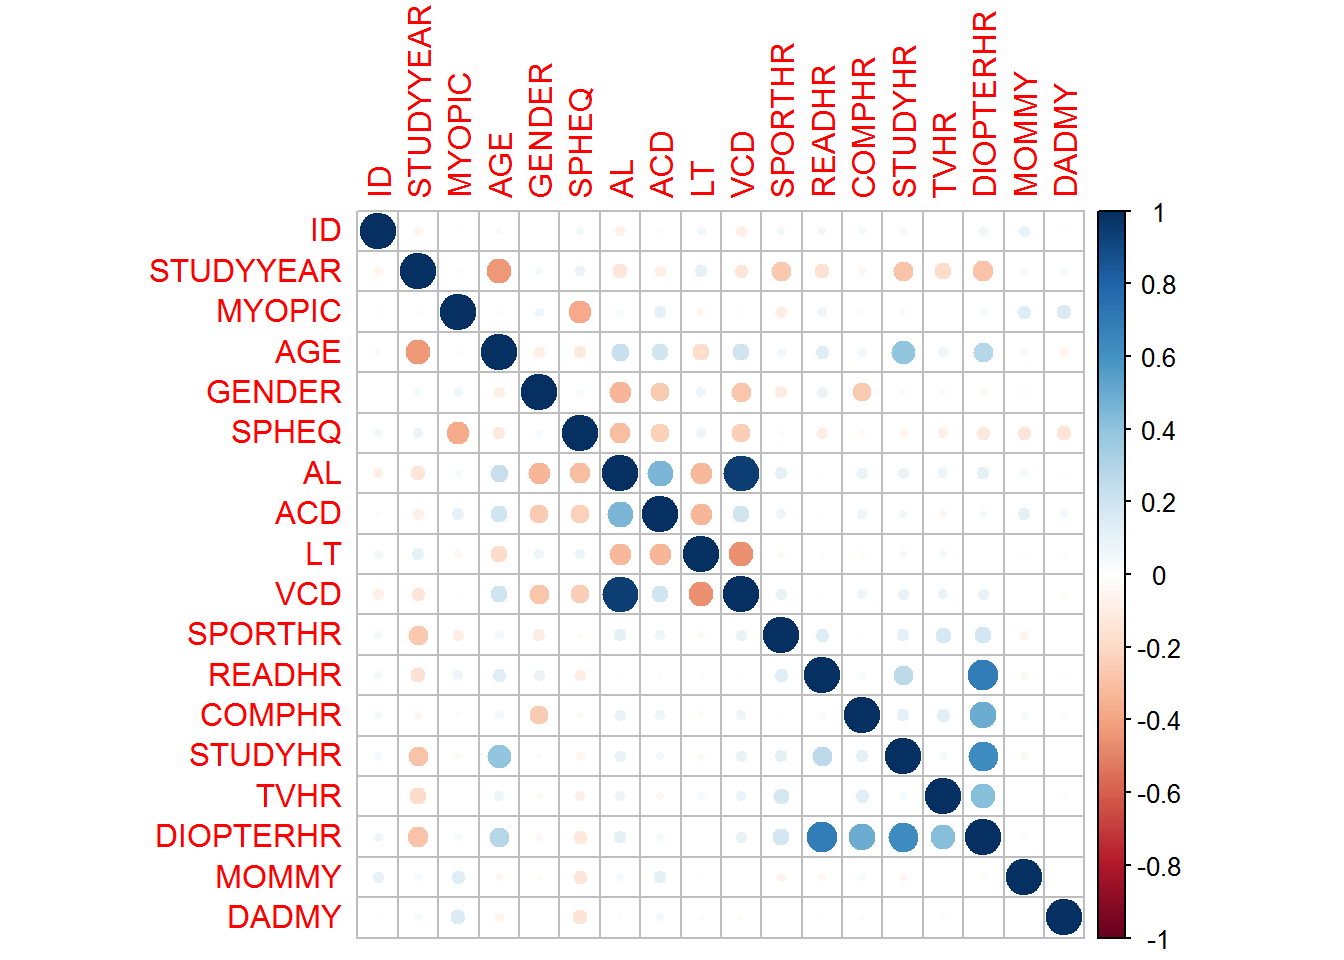
\includegraphics{02-foo_files/figure-latex/unnamed-chunk-3-2.pdf}
很明显,例如``DIOPTERHR''与``SPORTHR''、``TVHR''、``STUDYHR''、``COMPHR''和``READHR''高度相关。因此,``DIOPTERHR''变量不会包含在预测模型中 为了防止共线性问题

\hypertarget{ux53d8ux91cfux4e0eux8fd1ux89c6ux4e4bux95f4ux7684ux76f8ux5173ux6027}{%
\section{变量与近视之间的相关性}\label{ux53d8ux91cfux4e0eux8fd1ux89c6ux4e4bux95f4ux7684ux76f8ux5173ux6027}}

再来看每个属性与近视的关联性如何

\begin{Shaded}
\begin{Highlighting}[]
\FunctionTok{library}\NormalTok{(corrplot)}
\NormalTok{correlations }\OtherTok{\textless{}{-}} \FunctionTok{cor}\NormalTok{(data) }

\NormalTok{pcor }\OtherTok{\textless{}{-}}\NormalTok{ correlations[,}\DecValTok{3}\NormalTok{] }\SpecialCharTok{\%\textgreater{}\%} 
  \FunctionTok{print}\NormalTok{()}
\end{Highlighting}
\end{Shaded}

\begin{verbatim}
##           ID    STUDYYEAR       MYOPIC          AGE       GENDER        SPHEQ 
##  0.012242256  0.016330987  1.000000000  0.018525875  0.061556801 -0.373639054 
##           AL          ACD           LT          VCD      SPORTHR       READHR 
##  0.037752311  0.107952757 -0.045704451  0.011854862 -0.098282028  0.072749265 
##       COMPHR      STUDYHR         TVHR    DIOPTERHR        MOMMY        DADMY 
##  0.025874323 -0.031858867 -0.004032443  0.036983991  0.134032827  0.149896423
\end{verbatim}

\begin{Shaded}
\begin{Highlighting}[]
 \CommentTok{\# corrplot(correlations)}
\end{Highlighting}
\end{Shaded}

根据图中与近视高度相关的属性是``SPHEQ''、``ACD''、``MOMMY''、``DADMY''、``SPORTHR''、``READHR''、``GENDER''。

\hypertarget{ux53d8ux91cfux7b5bux9009}{%
\chapter{变量筛选}\label{ux53d8ux91cfux7b5bux9009}}

\hypertarget{ux5148ux5355ux540eux591a}{%
\section{先单后多}\label{ux5148ux5355ux540eux591a}}

\hypertarget{ux5206ux7c7bux53d8ux91cfux5904ux7406}{%
\subsection{分类变量处理}\label{ux5206ux7c7bux53d8ux91cfux5904ux7406}}

\begin{Shaded}
\begin{Highlighting}[]
\NormalTok{data }\OtherTok{\textless{}{-}} \FunctionTok{read.csv}\NormalTok{(}\StringTok{\textquotesingle{}myopia.csv\textquotesingle{}}\NormalTok{)}
\NormalTok{data}\SpecialCharTok{$}\NormalTok{MYOPIC }\OtherTok{\textless{}{-}} \FunctionTok{factor}\NormalTok{(data}\SpecialCharTok{$}\NormalTok{MYOPIC,}\AttributeTok{levels =} \FunctionTok{c}\NormalTok{(}\DecValTok{0}\NormalTok{,}\DecValTok{1}\NormalTok{),}\AttributeTok{labels =} \FunctionTok{c}\NormalTok{(}\StringTok{"非近视"}\NormalTok{,}\StringTok{"近视"}\NormalTok{))}
\NormalTok{data}\SpecialCharTok{$}\NormalTok{GENDER }\OtherTok{\textless{}{-}} \FunctionTok{factor}\NormalTok{(data}\SpecialCharTok{$}\NormalTok{GENDER,}\AttributeTok{levels =} \FunctionTok{c}\NormalTok{(}\DecValTok{0}\NormalTok{,}\DecValTok{1}\NormalTok{),}\AttributeTok{labels =} \FunctionTok{c}\NormalTok{(}\StringTok{"女性"}\NormalTok{,}\StringTok{"男性"}\NormalTok{))}
\NormalTok{data}\SpecialCharTok{$}\NormalTok{MOMMY }\OtherTok{\textless{}{-}} \FunctionTok{factor}\NormalTok{(data}\SpecialCharTok{$}\NormalTok{MOMMY,}\AttributeTok{levels =} \FunctionTok{c}\NormalTok{(}\DecValTok{0}\NormalTok{,}\DecValTok{1}\NormalTok{),}\AttributeTok{labels =} \FunctionTok{c}\NormalTok{(}\StringTok{"母亲不近视"}\NormalTok{,}\StringTok{"母亲近视"}\NormalTok{))}
\NormalTok{data}\SpecialCharTok{$}\NormalTok{DADMY }\OtherTok{\textless{}{-}} \FunctionTok{factor}\NormalTok{(data}\SpecialCharTok{$}\NormalTok{DADMY,}\AttributeTok{levels =} \FunctionTok{c}\NormalTok{(}\DecValTok{0}\NormalTok{,}\DecValTok{1}\NormalTok{),}\AttributeTok{labels =} \FunctionTok{c}\NormalTok{(}\StringTok{"父亲不近视"}\NormalTok{,}\StringTok{"父亲近视"}\NormalTok{))}
\CommentTok{\#年龄不设标签}
\CommentTok{\# str(data)}
\CommentTok{\# summary(data)}
\end{Highlighting}
\end{Shaded}

\hypertarget{ux5236ux4f5ctable1}{%
\subsection{制作table1}\label{ux5236ux4f5ctable1}}

\begin{Shaded}
\begin{Highlighting}[]
\CommentTok{\#连续性自变量}
\NormalTok{x1 }\OtherTok{\textless{}{-}} \FunctionTok{c}\NormalTok{(}\StringTok{"SPHEQ"}\NormalTok{,}\StringTok{"AL"}\NormalTok{,}\StringTok{"ACD"}\NormalTok{,}\StringTok{"LT"}\NormalTok{,}\StringTok{"VCD"}\NormalTok{,}\StringTok{"SPORTHR"}\NormalTok{,}\StringTok{"READHR"}\NormalTok{,}\StringTok{"COMPHR"}\NormalTok{,}\StringTok{"STUDYHR"}\NormalTok{,}\StringTok{"TVHR"}\NormalTok{,}\StringTok{"DIOPTERHR"}\NormalTok{)}
\CommentTok{\#分类变量}
\NormalTok{x2 }\OtherTok{\textless{}{-}} \FunctionTok{c}\NormalTok{(}\StringTok{"MYOPIC"}\NormalTok{,}\StringTok{"AGE"}\NormalTok{,}\StringTok{"GENDER"}\NormalTok{,}\StringTok{"MOMMY"}\NormalTok{,}\StringTok{"DADMY"}\NormalTok{)}
\end{Highlighting}
\end{Shaded}

\begin{Shaded}
\begin{Highlighting}[]
\FunctionTok{library}\NormalTok{(tableone)}
\end{Highlighting}
\end{Shaded}

\begin{verbatim}
## Warning: 程辑包'tableone'是用R版本4.1.2 来建造的
\end{verbatim}

\begin{Shaded}
\begin{Highlighting}[]
\NormalTok{table1 }\OtherTok{\textless{}{-}} \FunctionTok{CreateTableOne}\NormalTok{(}\AttributeTok{vars =} \FunctionTok{c}\NormalTok{(x1,x2),}
                       \AttributeTok{data =}\NormalTok{ data,}
                       \AttributeTok{factorVars =}\NormalTok{ x2,}
                       \AttributeTok{strata=}\FunctionTok{c}\NormalTok{(}\StringTok{"MYOPIC"}\NormalTok{),}\AttributeTok{addOverall =}\NormalTok{ F)}
\end{Highlighting}
\end{Shaded}

\begin{verbatim}
## Warning: replacing previous import 'lifecycle::last_warnings' by
## 'rlang::last_warnings' when loading 'pillar'
\end{verbatim}

\begin{verbatim}
## Warning: replacing previous import 'lifecycle::last_warnings' by
## 'rlang::last_warnings' when loading 'hms'
\end{verbatim}

\begin{Shaded}
\begin{Highlighting}[]
\NormalTok{results1 }\OtherTok{\textless{}{-}} \FunctionTok{print}\NormalTok{(table1,}\AttributeTok{shouwAllLevels=}\ConstantTok{FALSE}\NormalTok{)}
\end{Highlighting}
\end{Shaded}

\begin{verbatim}
##                        Stratified by MYOPIC
##                         非近视        近视           p      test
##   n                       537            81                     
##   SPHEQ (mean (SD))      0.89 (0.60)   0.20 (0.40)   <0.001     
##   AL (mean (SD))        22.49 (0.69)  22.56 (0.61)    0.349     
##   ACD (mean (SD))        3.57 (0.23)   3.64 (0.20)    0.007     
##   LT (mean (SD))         3.54 (0.16)   3.52 (0.14)    0.257     
##   VCD (mean (SD))       15.37 (0.67)  15.40 (0.61)    0.769     
##   SPORTHR (mean (SD))   12.26 (7.93)   9.94 (8.00)    0.015     
##   READHR (mean (SD))     2.71 (2.97)   3.37 (3.62)    0.071     
##   COMPHR (mean (SD))     2.07 (2.99)   2.31 (3.50)    0.521     
##   STUDYHR (mean (SD))    1.52 (2.29)   1.31 (1.68)    0.429     
##   TVHR (mean (SD))       8.96 (5.79)   8.89 (5.26)    0.920     
##   DIOPTERHR (mean (SD)) 25.79 (15.92) 27.54 (16.75)   0.359     
##   MYOPIC = 近视 (%)         0 ( 0.0)     81 (100.0)  <0.001     
##   AGE (%)                                             0.497     
##      5                     17 ( 3.2)      4 (  4.9)             
##      6                    398 (74.1)     58 ( 71.6)             
##      7                     73 (13.6)      9 ( 11.1)             
##      8                     45 ( 8.4)      8 (  9.9)             
##      9                      4 ( 0.7)      2 (  2.5)             
##   GENDER = 男性 (%)       256 (47.7)     46 ( 56.8)   0.158     
##   MOMMY = 母亲近视 (%)    258 (48.0)     55 ( 67.9)   0.001     
##   DADMY = 父亲近视 (%)    252 (46.9)     56 ( 69.1)  <0.001
\end{verbatim}

\begin{Shaded}
\begin{Highlighting}[]
\FunctionTok{write.csv}\NormalTok{(results1,}\StringTok{"table1.csv"}\NormalTok{)}
\end{Highlighting}
\end{Shaded}

\begin{Shaded}
\begin{Highlighting}[]
\CommentTok{\#如果不服从正态分布秩和检验、卡方检验}
\FunctionTok{library}\NormalTok{(tableone)}
\NormalTok{table1 }\OtherTok{\textless{}{-}} \FunctionTok{CreateTableOne}\NormalTok{(}\AttributeTok{vars =} \FunctionTok{c}\NormalTok{(x1,x2),}
                       \AttributeTok{data =}\NormalTok{ data,}
                       \AttributeTok{factorVars =}\NormalTok{ x2,}
                       \AttributeTok{strata =} \StringTok{"MYOPIC"}\NormalTok{,}\AttributeTok{addOverall =}\NormalTok{ F)}
\NormalTok{results2 }\OtherTok{\textless{}{-}} \FunctionTok{print}\NormalTok{(table1,}\AttributeTok{shouwAllLevels=}\ConstantTok{FALSE}\NormalTok{,}
                  \AttributeTok{nonnormal=}\NormalTok{x1)}\CommentTok{\#指定非阐述检验的变量}
\end{Highlighting}
\end{Shaded}

\begin{verbatim}
##                           Stratified by MYOPIC
##                            非近视               近视                 p     
##   n                          537                   81                      
##   SPHEQ (median [IQR])      0.79 [0.55, 1.10]    0.23 [-0.07, 0.50]  <0.001
##   AL (median [IQR])        22.45 [22.02, 22.97] 22.56 [22.07, 22.94]  0.360
##   ACD (median [IQR])        3.57 [3.41, 3.72]    3.68 [3.50, 3.74]    0.003
##   LT (median [IQR])         3.54 [3.44, 3.65]    3.51 [3.42, 3.63]    0.206
##   VCD (median [IQR])       15.36 [14.92, 15.83] 15.33 [14.96, 15.89]  0.741
##   SPORTHR (median [IQR])   10.00 [6.00, 16.00]   8.00 [3.00, 15.00]   0.005
##   READHR (median [IQR])     2.00 [0.00, 4.00]    3.00 [1.00, 5.00]    0.102
##   COMPHR (median [IQR])     1.00 [0.00, 3.00]    1.00 [0.00, 3.00]    0.892
##   STUDYHR (median [IQR])    1.00 [0.00, 2.00]    1.00 [0.00, 2.00]    0.967
##   TVHR (median [IQR])       8.00 [4.00, 12.00]   8.00 [5.00, 12.00]   0.820
##   DIOPTERHR (median [IQR]) 22.00 [14.00, 34.00] 24.00 [16.00, 36.00]  0.317
##   MYOPIC = 近视 (%)            0 ( 0.0)            81 (100.0)        <0.001
##   AGE (%)                                                             0.497
##      5                        17 ( 3.2)             4 (  4.9)              
##      6                       398 (74.1)            58 ( 71.6)              
##      7                        73 (13.6)             9 ( 11.1)              
##      8                        45 ( 8.4)             8 (  9.9)              
##      9                         4 ( 0.7)             2 (  2.5)              
##   GENDER = 男性 (%)          256 (47.7)            46 ( 56.8)         0.158
##   MOMMY = 母亲近视 (%)       258 (48.0)            55 ( 67.9)         0.001
##   DADMY = 父亲近视 (%)       252 (46.9)            56 ( 69.1)        <0.001
##                           Stratified by MYOPIC
##                            test   
##   n                               
##   SPHEQ (median [IQR])     nonnorm
##   AL (median [IQR])        nonnorm
##   ACD (median [IQR])       nonnorm
##   LT (median [IQR])        nonnorm
##   VCD (median [IQR])       nonnorm
##   SPORTHR (median [IQR])   nonnorm
##   READHR (median [IQR])    nonnorm
##   COMPHR (median [IQR])    nonnorm
##   STUDYHR (median [IQR])   nonnorm
##   TVHR (median [IQR])      nonnorm
##   DIOPTERHR (median [IQR]) nonnorm
##   MYOPIC = 近视 (%)               
##   AGE (%)                         
##      5                            
##      6                            
##      7                            
##      8                            
##      9                            
##   GENDER = 男性 (%)               
##   MOMMY = 母亲近视 (%)            
##   DADMY = 父亲近视 (%)
\end{verbatim}

\begin{Shaded}
\begin{Highlighting}[]
\CommentTok{\#exact 可以指定确切概论检验的变量,这里忽略(数据大,不需要)}
\FunctionTok{write.csv}\NormalTok{(results2,}\StringTok{"results2.csv"}\NormalTok{)}
\end{Highlighting}
\end{Shaded}

\hypertarget{ux5355ux56e0ux7d20logistic}{%
\subsection{单因素logistic}\label{ux5355ux56e0ux7d20logistic}}

\begin{Shaded}
\begin{Highlighting}[]
\CommentTok{\# 自变量}
\NormalTok{model }\OtherTok{\textless{}{-}} \FunctionTok{glm}\NormalTok{(MYOPIC }\SpecialCharTok{\textasciitilde{}}\NormalTok{ SPHEQ,}\AttributeTok{data =}\NormalTok{ data,}\AttributeTok{family =} \FunctionTok{binomial}\NormalTok{())}
\CommentTok{\# 查看模型结果}
\FunctionTok{summary}\NormalTok{(model)}\SpecialCharTok{$}\NormalTok{coefficients}
\end{Highlighting}
\end{Shaded}

\begin{verbatim}
##                Estimate Std. Error    z value     Pr(>|z|)
## (Intercept)  0.05397315  0.2067483  0.2610573 7.940483e-01
## SPHEQ       -3.83309762  0.4183696 -9.1619878 5.094998e-20
\end{verbatim}

\begin{Shaded}
\begin{Highlighting}[]
\CommentTok{\# 计算OR及其可信区间}
\FunctionTok{exp}\NormalTok{(}\FunctionTok{cbind}\NormalTok{(}\StringTok{"OR"}\OtherTok{=}\FunctionTok{coef}\NormalTok{(model),}\FunctionTok{confint}\NormalTok{(model)))}
\end{Highlighting}
\end{Shaded}

\begin{verbatim}
## Waiting for profiling to be done...
\end{verbatim}

\begin{verbatim}
##                     OR      2.5 %     97.5 %
## (Intercept) 1.05545626 0.70776986 1.59472261
## SPHEQ       0.02164247 0.00910867 0.04716271
\end{verbatim}

取单因素P\textless0.1

\hypertarget{ux591aux56e0ux7d20ux6a21ux578b}{%
\subsection{多因素模型}\label{ux591aux56e0ux7d20ux6a21ux578b}}

\begin{Shaded}
\begin{Highlighting}[]
\CommentTok{\# 多因素模型}
\NormalTok{model\_1}\OtherTok{\textless{}{-}} \FunctionTok{glm}\NormalTok{(}\FunctionTok{factor}\NormalTok{(MYOPIC)}\SpecialCharTok{\textasciitilde{}}\NormalTok{MOMMY}\SpecialCharTok{+}\NormalTok{DADMY}\SpecialCharTok{+}\NormalTok{SPHEQ}\SpecialCharTok{+}\NormalTok{ACD}\SpecialCharTok{+}\NormalTok{SPORTHR}\SpecialCharTok{+}\NormalTok{READHR,}\AttributeTok{family =} \StringTok{"binomial"}\NormalTok{,}\AttributeTok{data =}\NormalTok{ data)}
\CommentTok{\# 查看结果}
\FunctionTok{summary}\NormalTok{(model\_1)}\SpecialCharTok{$}\NormalTok{coefficients}
\end{Highlighting}
\end{Shaded}

\begin{verbatim}
##                  Estimate Std. Error   z value     Pr(>|z|)
## (Intercept)   -3.53288934 2.42831871 -1.454871 1.457051e-01
## MOMMY母亲近视  0.74791347 0.31126257  2.402838 1.626840e-02
## DADMY父亲近视  0.86552437 0.30735580  2.816034 4.862053e-03
## SPHEQ         -3.79733834 0.43556193 -8.718251 2.825317e-18
## ACD            0.82711271 0.66485466  1.244050 2.134810e-01
## SPORTHR       -0.05461693 0.02041790 -2.674953 7.473971e-03
## READHR         0.06843900 0.04577874  1.494995 1.349157e-01
\end{verbatim}

\begin{Shaded}
\begin{Highlighting}[]
\CommentTok{\# 计算OR及其可信区间}
\FunctionTok{exp}\NormalTok{(}\FunctionTok{cbind}\NormalTok{(}\StringTok{"OR"}\OtherTok{=}\FunctionTok{coef}\NormalTok{(model),}\FunctionTok{confint}\NormalTok{(model\_1)))}
\end{Highlighting}
\end{Shaded}

\begin{verbatim}
## Waiting for profiling to be done...
\end{verbatim}

\begin{verbatim}
## Warning in cbind(OR = coef(model), confint(model_1)): number of rows of result
## is not a multiple of vector length (arg 1)
\end{verbatim}

\begin{verbatim}
##                       OR        2.5 %     97.5 %
## (Intercept)   1.05545626 0.0002380046 3.33425391
## MOMMY母亲近视 0.02164247 1.1604118328 3.95048116
## DADMY父亲近视 1.05545626 1.3157000566 4.41021361
## SPHEQ         0.02164247 0.0090945183 0.05041805
## ACD           1.05545626 0.6237053229 8.51268747
## SPORTHR       0.02164247 0.9077904406 0.98385439
## READHR        1.05545626 0.9784535086 1.17140573
\end{verbatim}

\hypertarget{ps-ux5f15ux5165ux53d8ux91cf}{%
\subsubsection{PS: 引入变量}\label{ps-ux5f15ux5165ux53d8ux91cf}}

如果我们已经确定是研究自变量X 与 因变量Y之间的关系,这时候协变量应该如何筛选进入多因素模型呢?
如果某个协变量Z与因变量Y之间单因素分析的P值小于0.1,并且协变量Z与自变量X同时分析与因变量Y的关系,由于Z的存在,使X的系数较单因素分析时变化超过10\%,这时候协变量Z应该纳入多因素分析中。

我们这里主要(关心)的X 变量时SPHEQ情况,其他自变量都是协变量Z

\begin{Shaded}
\begin{Highlighting}[]
\NormalTok{uni\_methods}\OtherTok{\textless{}{-}}\ControlFlowTok{function}\NormalTok{(xvar)\{}
\NormalTok{  model}\OtherTok{\textless{}{-}}\FunctionTok{glm}\NormalTok{(MYOPIC}\SpecialCharTok{\textasciitilde{}}\NormalTok{SPHEQ,}\AttributeTok{data =}\NormalTok{ data,}\AttributeTok{family =} \FunctionTok{binomial}\NormalTok{())}
\NormalTok{  coef }\OtherTok{\textless{}{-}} \FunctionTok{coef}\NormalTok{(model)[}\DecValTok{2}\NormalTok{]}
\NormalTok{  form }\OtherTok{\textless{}{-}} \FunctionTok{as.formula}\NormalTok{(}\FunctionTok{paste0}\NormalTok{(}\StringTok{"MYOPIC\textasciitilde{}SPHEQ+"}\NormalTok{,xvar))}
\NormalTok{  model2 }\OtherTok{\textless{}{-}} \FunctionTok{glm}\NormalTok{(form,}\AttributeTok{data =}\NormalTok{ data,}\AttributeTok{family =} \FunctionTok{binomial}\NormalTok{())}
\NormalTok{  coef2 }\OtherTok{\textless{}{-}} \FunctionTok{coef}\NormalTok{(model2)[}\DecValTok{2}\NormalTok{]}
\NormalTok{  ratio }\OtherTok{\textless{}{-}} \FunctionTok{abs}\NormalTok{(coef2}\SpecialCharTok{{-}}\NormalTok{coef)}\SpecialCharTok{/}\NormalTok{coef}\SpecialCharTok{\textgreater{}}\FloatTok{0.1}
  \ControlFlowTok{if}\NormalTok{(ratio)\{}
    \FunctionTok{return}\NormalTok{(xvar)}
\NormalTok{  \}}
\NormalTok{\}}
\end{Highlighting}
\end{Shaded}

\begin{Shaded}
\begin{Highlighting}[]
\NormalTok{xvar }\OtherTok{\textless{}{-}} \FunctionTok{c}\NormalTok{(x1,x2)}
\NormalTok{xvar }\OtherTok{\textless{}{-}}\NormalTok{ xvar[}\SpecialCharTok{{-}}\FunctionTok{which}\NormalTok{(xvar}\SpecialCharTok{==}\StringTok{"SPHEQ"}\NormalTok{)]}
\NormalTok{xvar}
\end{Highlighting}
\end{Shaded}

\begin{verbatim}
##  [1] "AL"        "ACD"       "LT"        "VCD"       "SPORTHR"   "READHR"   
##  [7] "COMPHR"    "STUDYHR"   "TVHR"      "DIOPTERHR" "MYOPIC"    "AGE"      
## [13] "GENDER"    "MOMMY"     "DADMY"
\end{verbatim}

\begin{Shaded}
\begin{Highlighting}[]
\FunctionTok{lapply}\NormalTok{(xvar,uni\_methods)}
\end{Highlighting}
\end{Shaded}

\begin{verbatim}
## Warning in model.matrix.default(mt, mf, contrasts): 在公式右手的反应略过不用
\end{verbatim}

\begin{verbatim}
## Warning in model.matrix.default(mt, mf, contrasts): 模型矩阵的2项有问题: 没有指
## 定的列
\end{verbatim}

\begin{verbatim}
## [[1]]
## NULL
## 
## [[2]]
## NULL
## 
## [[3]]
## NULL
## 
## [[4]]
## NULL
## 
## [[5]]
## NULL
## 
## [[6]]
## NULL
## 
## [[7]]
## NULL
## 
## [[8]]
## NULL
## 
## [[9]]
## NULL
## 
## [[10]]
## NULL
## 
## [[11]]
## NULL
## 
## [[12]]
## NULL
## 
## [[13]]
## NULL
## 
## [[14]]
## NULL
## 
## [[15]]
## NULL
\end{verbatim}

\hypertarget{lasso-logistic}{%
\chapter{LASSO-Logistic}\label{lasso-logistic}}

\emph{lasso 回归不能把数据处理成factor,如果涉及多分类,手动设置哑变量}

\hypertarget{ux8bfbux5165ux6570ux636e}{%
\section{读入数据}\label{ux8bfbux5165ux6570ux636e}}

\begin{Shaded}
\begin{Highlighting}[]
\FunctionTok{library}\NormalTok{(tidyverse)}
\end{Highlighting}
\end{Shaded}

\begin{verbatim}
## Warning: replacing previous import 'lifecycle::last_warnings' by
## 'rlang::last_warnings' when loading 'pillar'
\end{verbatim}

\begin{verbatim}
## Warning: replacing previous import 'lifecycle::last_warnings' by
## 'rlang::last_warnings' when loading 'hms'
\end{verbatim}

\begin{verbatim}
## -- Attaching packages --------------------------------------- tidyverse 1.3.1 --
\end{verbatim}

\begin{verbatim}
## v ggplot2 3.3.5     v purrr   0.3.4
## v tibble  3.1.7     v dplyr   1.0.7
## v tidyr   1.1.3     v stringr 1.4.0
## v readr   2.0.1     v forcats 0.5.1
\end{verbatim}

\begin{verbatim}
## Warning: 程辑包'tibble'是用R版本4.1.3 来建造的
\end{verbatim}

\begin{verbatim}
## -- Conflicts ------------------------------------------ tidyverse_conflicts() --
## x dplyr::filter() masks stats::filter()
## x dplyr::lag()    masks stats::lag()
\end{verbatim}

\begin{Shaded}
\begin{Highlighting}[]
\NormalTok{myopia }\OtherTok{\textless{}{-}} \FunctionTok{read.csv}\NormalTok{(}\StringTok{"myopia.csv"}\NormalTok{) }\SpecialCharTok{\%\textgreater{}\%} 
  \FunctionTok{mutate}\NormalTok{(}\AttributeTok{PARENTS=}\NormalTok{MOMMY}\SpecialCharTok{+}\NormalTok{DADMY) }\SpecialCharTok{\%\textgreater{}\%} 
  \FunctionTok{select}\NormalTok{(ID}\SpecialCharTok{:}\NormalTok{DIOPTERHR,PARENTS)}
\end{Highlighting}
\end{Shaded}

\hypertarget{ux5c06ux6570ux636eux96c6ux5206ux6210ux8badux7ec3ux96c6ux548cux6d4bux8bd5ux96c6}{%
\section{将数据集分成训练集和测试集}\label{ux5c06ux6570ux636eux96c6ux5206ux6210ux8badux7ec3ux96c6ux548cux6d4bux8bd5ux96c6}}

\begin{Shaded}
\begin{Highlighting}[]
\FunctionTok{library}\NormalTok{(caret)}
\end{Highlighting}
\end{Shaded}

\begin{verbatim}
## Warning: 程辑包'caret'是用R版本4.1.3 来建造的
\end{verbatim}

\begin{verbatim}
## 载入需要的程辑包:lattice
\end{verbatim}

\begin{verbatim}
## 
## 载入程辑包:'caret'
\end{verbatim}

\begin{verbatim}
## The following object is masked from 'package:purrr':
## 
##     lift
\end{verbatim}

\begin{Shaded}
\begin{Highlighting}[]
\FunctionTok{set.seed}\NormalTok{(}\DecValTok{1000}\NormalTok{)}
\NormalTok{index }\OtherTok{\textless{}{-}} \FunctionTok{createDataPartition}\NormalTok{(}
\NormalTok{  myopia}\SpecialCharTok{$}\NormalTok{MYOPIC,}
  \AttributeTok{p =} \FloatTok{0.7}\NormalTok{,}
  \AttributeTok{list =} \ConstantTok{FALSE}
\NormalTok{)}
\NormalTok{train }\OtherTok{\textless{}{-}}\NormalTok{ myopia[index, ]}
\NormalTok{test }\OtherTok{\textless{}{-}}\NormalTok{ myopia[}\SpecialCharTok{{-}}\NormalTok{index, ]}
\end{Highlighting}
\end{Shaded}

\hypertarget{ux52a0ux8f7dux5305}{%
\section{加载包}\label{ux52a0ux8f7dux5305}}

\begin{Shaded}
\begin{Highlighting}[]
\FunctionTok{library}\NormalTok{(corrplot)}
\end{Highlighting}
\end{Shaded}

\begin{verbatim}
## Warning: 程辑包'corrplot'是用R版本4.1.2 来建造的
\end{verbatim}

\begin{verbatim}
## corrplot 0.92 loaded
\end{verbatim}

\begin{Shaded}
\begin{Highlighting}[]
\FunctionTok{library}\NormalTok{(car)}
\end{Highlighting}
\end{Shaded}

\begin{verbatim}
## 载入需要的程辑包:carData
\end{verbatim}

\begin{verbatim}
## 
## 载入程辑包:'car'
\end{verbatim}

\begin{verbatim}
## The following object is masked from 'package:dplyr':
## 
##     recode
\end{verbatim}

\begin{verbatim}
## The following object is masked from 'package:purrr':
## 
##     some
\end{verbatim}

\begin{Shaded}
\begin{Highlighting}[]
\FunctionTok{library}\NormalTok{(leaps)}
\end{Highlighting}
\end{Shaded}

\begin{verbatim}
## Warning: 程辑包'leaps'是用R版本4.1.3 来建造的
\end{verbatim}

\begin{Shaded}
\begin{Highlighting}[]
\FunctionTok{library}\NormalTok{(glmnet)}\CommentTok{\#岭回归、lasso、弹性网络模型}
\end{Highlighting}
\end{Shaded}

\begin{verbatim}
## Warning: 程辑包'glmnet'是用R版本4.1.2 来建造的
\end{verbatim}

\begin{verbatim}
## 载入需要的程辑包:Matrix
\end{verbatim}

\begin{verbatim}
## 
## 载入程辑包:'Matrix'
\end{verbatim}

\begin{verbatim}
## The following objects are masked from 'package:tidyr':
## 
##     expand, pack, unpack
\end{verbatim}

\begin{verbatim}
## Loaded glmnet 4.1-3
\end{verbatim}

\begin{Shaded}
\begin{Highlighting}[]
\FunctionTok{library}\NormalTok{(caret)}
\DocumentationTok{\#\#\#\# 在glmnet()语法中alpha=0为岭回归,alpha=1表示lasso回归}
\end{Highlighting}
\end{Shaded}

\begin{Shaded}
\begin{Highlighting}[]
\NormalTok{correlations }\OtherTok{\textless{}{-}} \FunctionTok{cor}\NormalTok{(myopia)}
\NormalTok{pcor }\OtherTok{\textless{}{-}}\NormalTok{ correlations[,}\DecValTok{3}\NormalTok{] }\SpecialCharTok{\%\textgreater{}\%}
  \FunctionTok{print}\NormalTok{()}
\end{Highlighting}
\end{Shaded}

\begin{verbatim}
##           ID    STUDYYEAR       MYOPIC          AGE       GENDER        SPHEQ 
##  0.012242256  0.016330987  1.000000000  0.018525875  0.061556801 -0.373639054 
##           AL          ACD           LT          VCD      SPORTHR       READHR 
##  0.037752311  0.107952757 -0.045704451  0.011854862 -0.098282028  0.072749265 
##       COMPHR      STUDYHR         TVHR    DIOPTERHR      PARENTS 
##  0.025874323 -0.031858867 -0.004032443  0.036983991  0.201417458
\end{verbatim}

\begin{Shaded}
\begin{Highlighting}[]
\FunctionTok{corrplot.mixed}\NormalTok{(}\FunctionTok{cor}\NormalTok{(myopia))}
\end{Highlighting}
\end{Shaded}

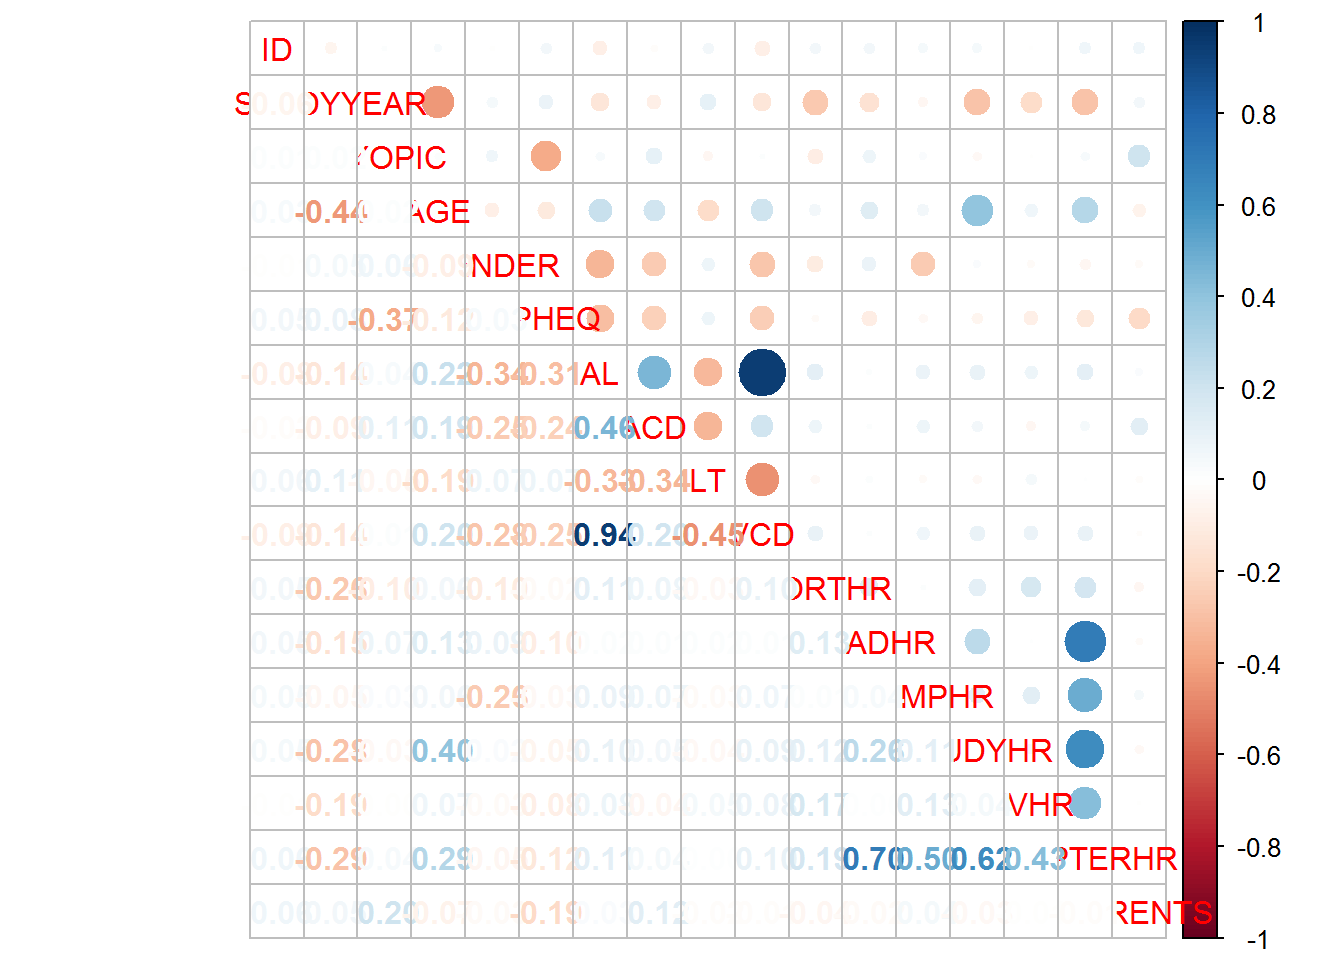
\includegraphics{04-lasso_files/figure-latex/unnamed-chunk-4-1.pdf}
``SPHEQ'', ``ACD'', '\,'MOMMY'', ``DADMY'', ''SPORTHR'' , ''READHR'',''GENDER''

\hypertarget{ux5b9aux4e49ux81eaux53d8ux91cfux56e0ux53d8ux91cf}{%
\section{定义自变量,因变量}\label{ux5b9aux4e49ux81eaux53d8ux91cfux56e0ux53d8ux91cf}}

\begin{Shaded}
\begin{Highlighting}[]
\NormalTok{x }\OtherTok{\textless{}{-}} \FunctionTok{as.matrix}\NormalTok{(train[,}\DecValTok{4}\SpecialCharTok{:}\DecValTok{17}\NormalTok{])}
\NormalTok{y }\OtherTok{\textless{}{-}}\NormalTok{ train[,}\DecValTok{3}\NormalTok{]}
\NormalTok{lambdas }\OtherTok{\textless{}{-}} \DecValTok{10} \SpecialCharTok{\^{}} \FunctionTok{seq}\NormalTok{(}\DecValTok{8}\NormalTok{,}\SpecialCharTok{{-}}\DecValTok{4}\NormalTok{,}\AttributeTok{length=}\DecValTok{250}\NormalTok{)}
\end{Highlighting}
\end{Shaded}

\hypertarget{section}{%
\chapter{}\label{section}}

\begin{Shaded}
\begin{Highlighting}[]
\NormalTok{lasso }\OtherTok{\textless{}{-}} \FunctionTok{glmnet}\NormalTok{(x,y,}\AttributeTok{family =} \StringTok{"binomial"}\NormalTok{,}\AttributeTok{alpha =} \DecValTok{1}\NormalTok{)}
\FunctionTok{print}\NormalTok{(lasso)}
\end{Highlighting}
\end{Shaded}

\begin{verbatim}
## 
## Call:  glmnet(x = x, y = y, family = "binomial", alpha = 1) 
## 
##    Df  %Dev   Lambda
## 1   0  0.00 0.115200
## 2   1  2.76 0.105000
## 3   1  5.36 0.095630
## 4   1  7.78 0.087140
## 5   1  9.99 0.079400
## 6   1 11.99 0.072340
## 7   1 13.78 0.065920
## 8   1 15.35 0.060060
## 9   1 16.73 0.054720
## 10  2 18.06 0.049860
## 11  2 19.49 0.045430
## 12  2 20.74 0.041400
## 13  3 21.91 0.037720
## 14  3 23.02 0.034370
## 15  3 23.98 0.031320
## 16  4 24.92 0.028530
## 17  4 25.79 0.026000
## 18  4 26.54 0.023690
## 19  4 27.19 0.021580
## 20  4 27.75 0.019670
## 21  4 28.23 0.017920
## 22  4 28.64 0.016330
## 23  5 29.01 0.014880
## 24  8 29.43 0.013560
## 25  8 29.82 0.012350
## 26  8 30.15 0.011250
## 27  8 30.44 0.010250
## 28  9 30.73 0.009343
## 29 10 31.00 0.008513
## 30 11 31.26 0.007757
## 31 11 31.48 0.007068
## 32 11 31.68 0.006440
## 33 11 31.84 0.005868
## 34 12 31.99 0.005347
## 35 12 32.12 0.004872
## 36 12 32.23 0.004439
## 37 12 32.32 0.004045
## 38 12 32.40 0.003685
## 39 12 32.47 0.003358
## 40 12 32.53 0.003060
## 41 12 32.57 0.002788
## 42 12 32.61 0.002540
## 43 12 32.65 0.002314
## 44 12 32.68 0.002109
## 45 12 32.70 0.001921
## 46 12 32.72 0.001751
## 47 12 32.74 0.001595
## 48 12 32.75 0.001454
## 49 12 32.76 0.001324
## 50 12 32.77 0.001207
## 51 12 32.78 0.001100
## 52 12 32.79 0.001002
## 53 12 32.79 0.000913
## 54 12 32.80 0.000832
## 55 12 32.80 0.000758
## 56 12 32.81 0.000691
## 57 13 32.81 0.000629
## 58 13 32.81 0.000573
## 59 13 32.81 0.000522
## 60 13 32.81 0.000476
## 61 13 32.82 0.000434
## 62 13 32.82 0.000395
## 63 13 32.82 0.000360
\end{verbatim}

\begin{Shaded}
\begin{Highlighting}[]
\FunctionTok{plot}\NormalTok{(lasso,}\AttributeTok{xvar=}\StringTok{"lambda"}\NormalTok{,}\AttributeTok{label =} \ConstantTok{TRUE}\NormalTok{)}
\end{Highlighting}
\end{Shaded}

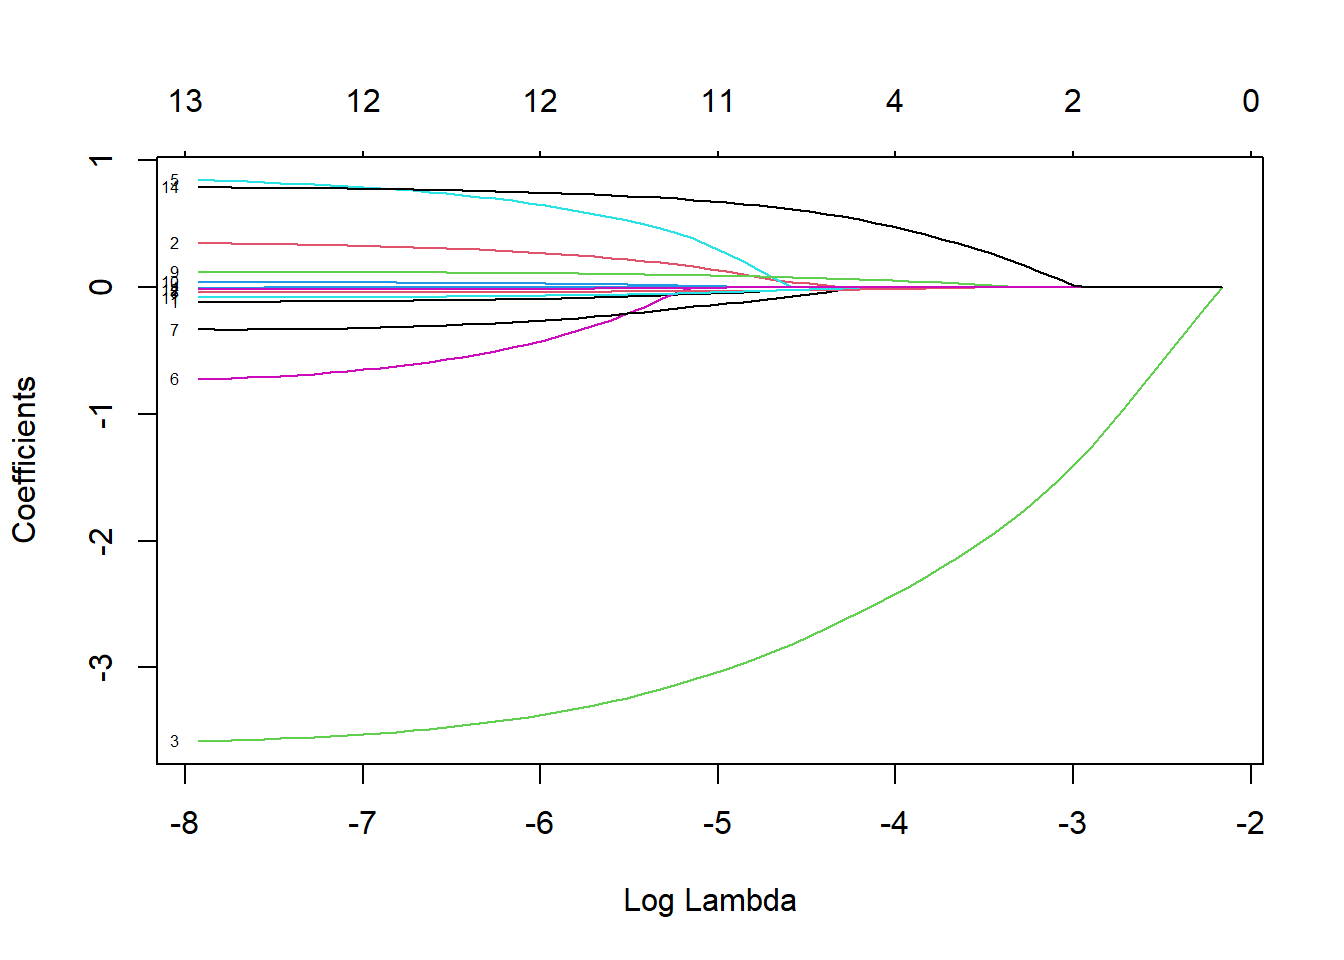
\includegraphics{04-lasso_files/figure-latex/unnamed-chunk-7-1.pdf}

传入一个lambda值看看

\begin{Shaded}
\begin{Highlighting}[]
\NormalTok{loss.coef }\OtherTok{\textless{}{-}} \FunctionTok{predict}\NormalTok{(lasso,}\AttributeTok{s=}\FloatTok{0.05}\NormalTok{,}\AttributeTok{type =} \StringTok{\textquotesingle{}coefficients\textquotesingle{}}\NormalTok{)}
\NormalTok{loss.coef}
\end{Highlighting}
\end{Shaded}

\begin{verbatim}
## 15 x 1 sparse Matrix of class "dgCMatrix"
##                      s1
## (Intercept) -1.04549610
## AGE          .         
## GENDER       .         
## SPHEQ       -1.40167370
## AL           .         
## ACD          .         
## LT           .         
## VCD          .         
## SPORTHR      .         
## READHR       .         
## COMPHR       .         
## STUDYHR      .         
## TVHR         .         
## DIOPTERHR    .         
## PARENTS      0.01645111
\end{verbatim}

type=c(``link'', ``response'', ``class'', ``coefficients'', ``nonzero'')。link给出的是线性预测值,即进行logit变化前的值,函数默认值;response给出的是概率预测值,即进行logit变换之后的值;clase给出0/1预测值;coefficients给出的是指定λ值的模型系数;nonzero给出指定的定λ值时系数不为0的模型变量。

\hypertarget{cvux4ea4ux53c9ux9a8cux8bc1}{%
\section{cv交叉验证}\label{cvux4ea4ux53c9ux9a8cux8bc1}}

\begin{Shaded}
\begin{Highlighting}[]
\NormalTok{lasso.cv }\OtherTok{\textless{}{-}} \FunctionTok{cv.glmnet}\NormalTok{(x,y, }\AttributeTok{alpha=}\DecValTok{1}\NormalTok{,  }\AttributeTok{family=}\StringTok{"binomial"}\NormalTok{)}
\FunctionTok{plot}\NormalTok{(lasso.cv)}
\end{Highlighting}
\end{Shaded}

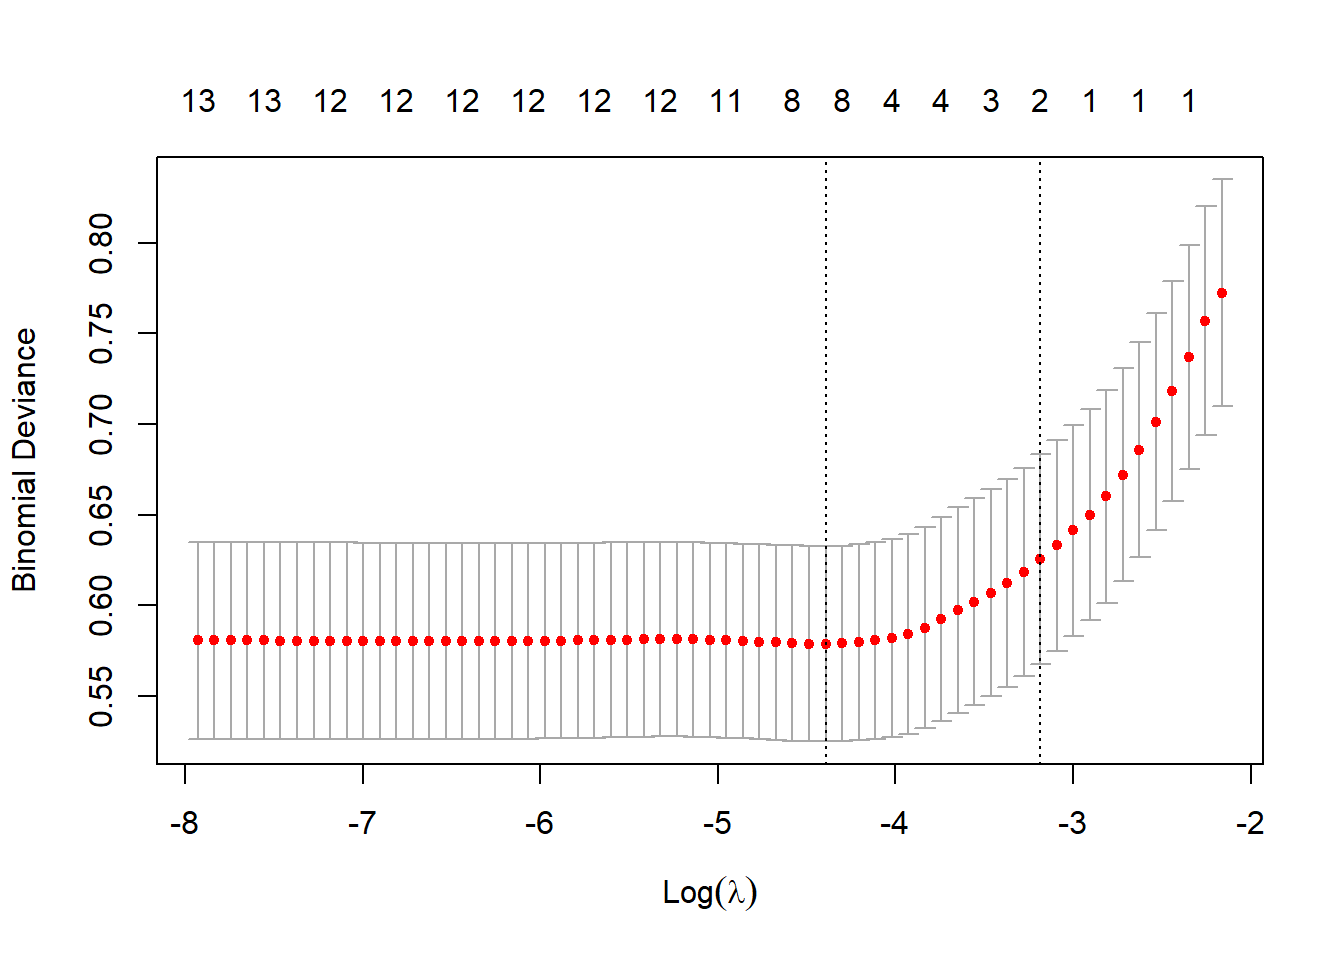
\includegraphics{04-lasso_files/figure-latex/unnamed-chunk-9-1.pdf}

\begin{Shaded}
\begin{Highlighting}[]
\NormalTok{lasso.cv\_auc }\OtherTok{\textless{}{-}} \FunctionTok{cv.glmnet}\NormalTok{(x,y,}\AttributeTok{alpha=}\DecValTok{1}\NormalTok{,}\AttributeTok{family=}\StringTok{"binomial"}\NormalTok{,}\AttributeTok{type.measure =} \StringTok{"auc"}\NormalTok{)}
\FunctionTok{plot}\NormalTok{(lasso.cv\_auc)}
\end{Highlighting}
\end{Shaded}

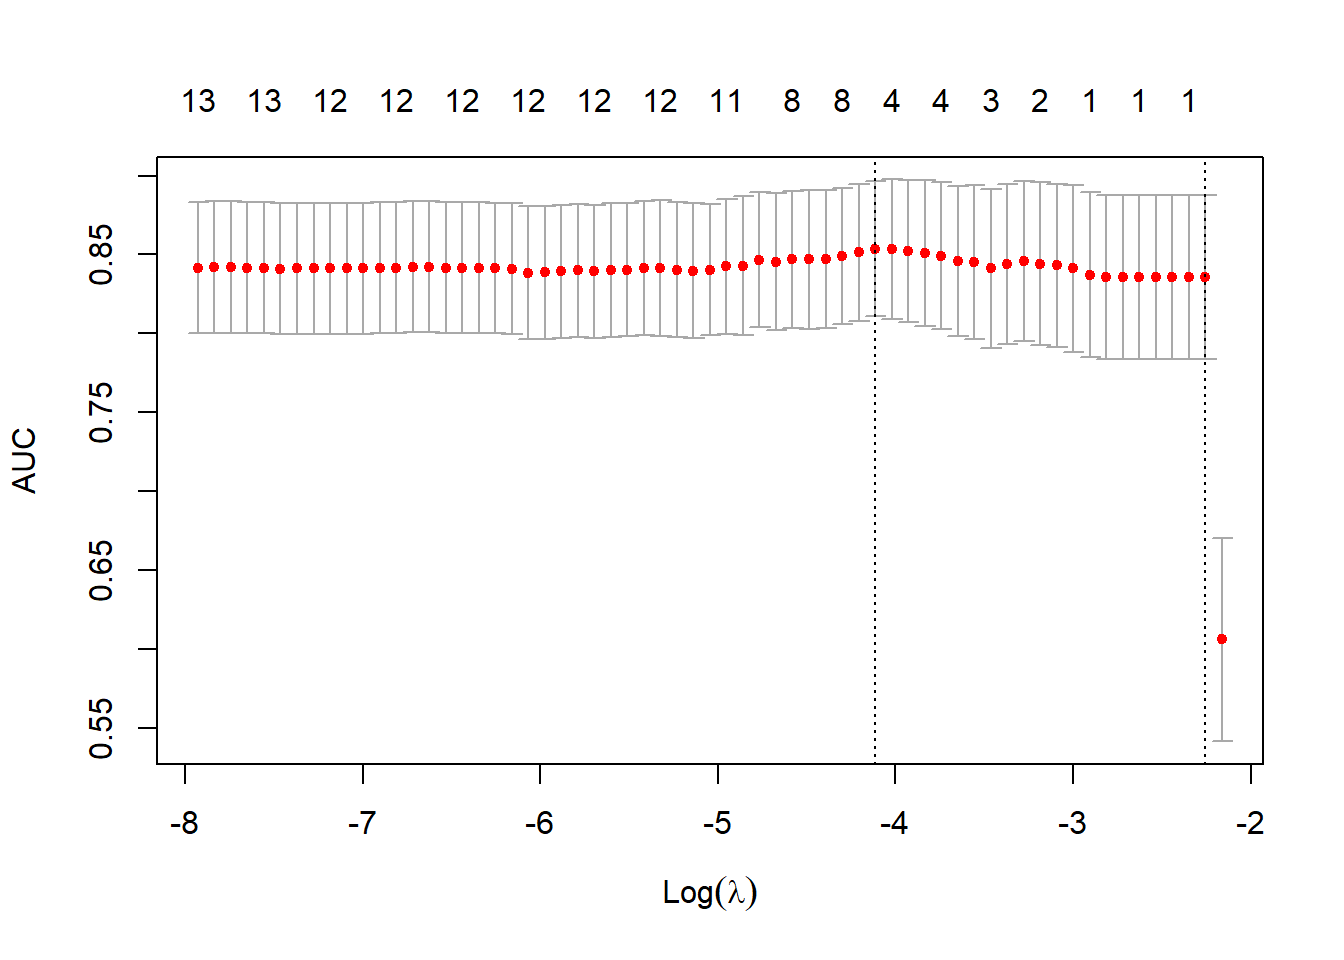
\includegraphics{04-lasso_files/figure-latex/unnamed-chunk-9-2.pdf}

横坐标是lambda的对数值,也就是惩罚力度,值越大,惩罚力度越大。纵坐标是模型的MSE(均方误差)。图形上方横坐标是自变量数量。随着lambda的增加,MSE不断变化。第一条虚线表示MSE最小值对应的lambda值,第二条虚线表示距离均方误差一个标准误时的lambda值(最优解)

\begin{Shaded}
\begin{Highlighting}[]
\FunctionTok{coef}\NormalTok{(lasso.cv , }\AttributeTok{s =} \FunctionTok{c}\NormalTok{(}\DecValTok{1}\NormalTok{,}\FloatTok{0.1}\NormalTok{,}\FloatTok{0.01}\NormalTok{,}\FloatTok{0.001}\NormalTok{))}
\end{Highlighting}
\end{Shaded}

\begin{verbatim}
## 15 x 4 sparse Matrix of class "dgCMatrix"
##                    s1         s2          s3          s4
## (Intercept) -1.906893 -1.7282362  0.16212541  4.02046678
## AGE          .         .         -0.02171082 -0.10849682
## GENDER       .         .          0.04626298  0.32335354
## SPHEQ        .        -0.2400235 -2.82801562 -3.51734389
## AL           .         .          .           .         
## ACD          .         .          0.01674432  0.78087139
## LT           .         .          .          -0.63712500
## VCD          .         .         -0.07605748 -0.31816768
## SPORTHR      .         .         -0.02514996 -0.03991801
## READHR       .         .          0.07966571  0.11800176
## COMPHR       .         .          .           0.03702366
## STUDYHR      .         .         -0.02353405 -0.07749223
## TVHR         .         .          .          -0.01674881
## DIOPTERHR    .         .          .           .         
## PARENTS      .         .          0.61989773  0.77437955
\end{verbatim}

\begin{Shaded}
\begin{Highlighting}[]
\NormalTok{lasso.cv\_min }\OtherTok{\textless{}{-}}\NormalTok{ lasso.cv}\SpecialCharTok{$}\NormalTok{lambda.min }\SpecialCharTok{\%\textgreater{}\%} 
  \FunctionTok{print}\NormalTok{()}
\end{Highlighting}
\end{Shaded}

\begin{verbatim}
## [1] 0.01235143
\end{verbatim}

\begin{Shaded}
\begin{Highlighting}[]
\NormalTok{lasso.coef }\OtherTok{\textless{}{-}} \FunctionTok{coef}\NormalTok{(lasso.cv}\SpecialCharTok{$}\NormalTok{glmnet.fit,}\AttributeTok{s=}\NormalTok{lasso.cv\_min,}\AttributeTok{exact =}\NormalTok{ F)}
\NormalTok{lasso.coef}
\end{Highlighting}
\end{Shaded}

\begin{verbatim}
## 15 x 1 sparse Matrix of class "dgCMatrix"
##                       s1
## (Intercept) -0.470162310
## AGE         -0.009058156
## GENDER       0.015668468
## SPHEQ       -2.694167376
## AL           .          
## ACD          .          
## LT           .          
## VCD         -0.036936193
## SPORTHR     -0.022001607
## READHR       0.071207248
## COMPHR       .          
## STUDYHR     -0.012574109
## TVHR         .          
## DIOPTERHR    .          
## PARENTS      0.577869537
\end{verbatim}

我们可以试一下如果选择1s是什么情况

\begin{Shaded}
\begin{Highlighting}[]
\NormalTok{lasso.cv\_1se }\OtherTok{\textless{}{-}}\NormalTok{ lasso.cv}\SpecialCharTok{$}\NormalTok{lambda}\FloatTok{.1}\NormalTok{se}\CommentTok{\#通常使用距离MSE最小一个标准差lambda作为最合适的,直接调用即可}

\NormalTok{lasso.coef\_1se}\OtherTok{\textless{}{-}} \FunctionTok{coef}\NormalTok{(lasso.cv}\SpecialCharTok{$}\NormalTok{glmnet.fit,}\AttributeTok{s=}\NormalTok{lasso.cv\_1se,}\AttributeTok{exact =}\NormalTok{ F)}
\NormalTok{lasso.coef\_1se}
\end{Highlighting}
\end{Shaded}

\begin{verbatim}
## 15 x 1 sparse Matrix of class "dgCMatrix"
##                     s1
## (Intercept) -1.0378542
## AGE          .        
## GENDER       .        
## SPHEQ       -1.6514186
## AL           .        
## ACD          .        
## LT           .        
## VCD          .        
## SPORTHR      .        
## READHR       .        
## COMPHR       .        
## STUDYHR      .        
## TVHR         .        
## DIOPTERHR    .        
## PARENTS      0.1220882
\end{verbatim}

\hypertarget{lassoux5728ux6d4bux8bd5ux96c6ux4e0aux7684ux8868ux73b0}{%
\section{lasso在测试集上的表现}\label{lassoux5728ux6d4bux8bd5ux96c6ux4e0aux7684ux8868ux73b0}}

\begin{Shaded}
\begin{Highlighting}[]
\NormalTok{newx}\OtherTok{=}\FunctionTok{as.matrix}\NormalTok{(test[}\DecValTok{4}\SpecialCharTok{:}\DecValTok{17}\NormalTok{])}
\NormalTok{lasso.y }\OtherTok{\textless{}{-}} \FunctionTok{predict}\NormalTok{(lasso,}\AttributeTok{newx =}\NormalTok{ newx,}\AttributeTok{type =} \StringTok{"response"}\NormalTok{,}\AttributeTok{s=}\FloatTok{0.01235}\NormalTok{)}
\FunctionTok{plot}\NormalTok{(lasso.y,test}\SpecialCharTok{$}\NormalTok{MYOPIC,}\AttributeTok{xlab=}\StringTok{"Predicted"}\NormalTok{,}\AttributeTok{ylab=}\StringTok{"Actual"}\NormalTok{,}\AttributeTok{main=}\StringTok{"lasso"}\NormalTok{)}
\end{Highlighting}
\end{Shaded}

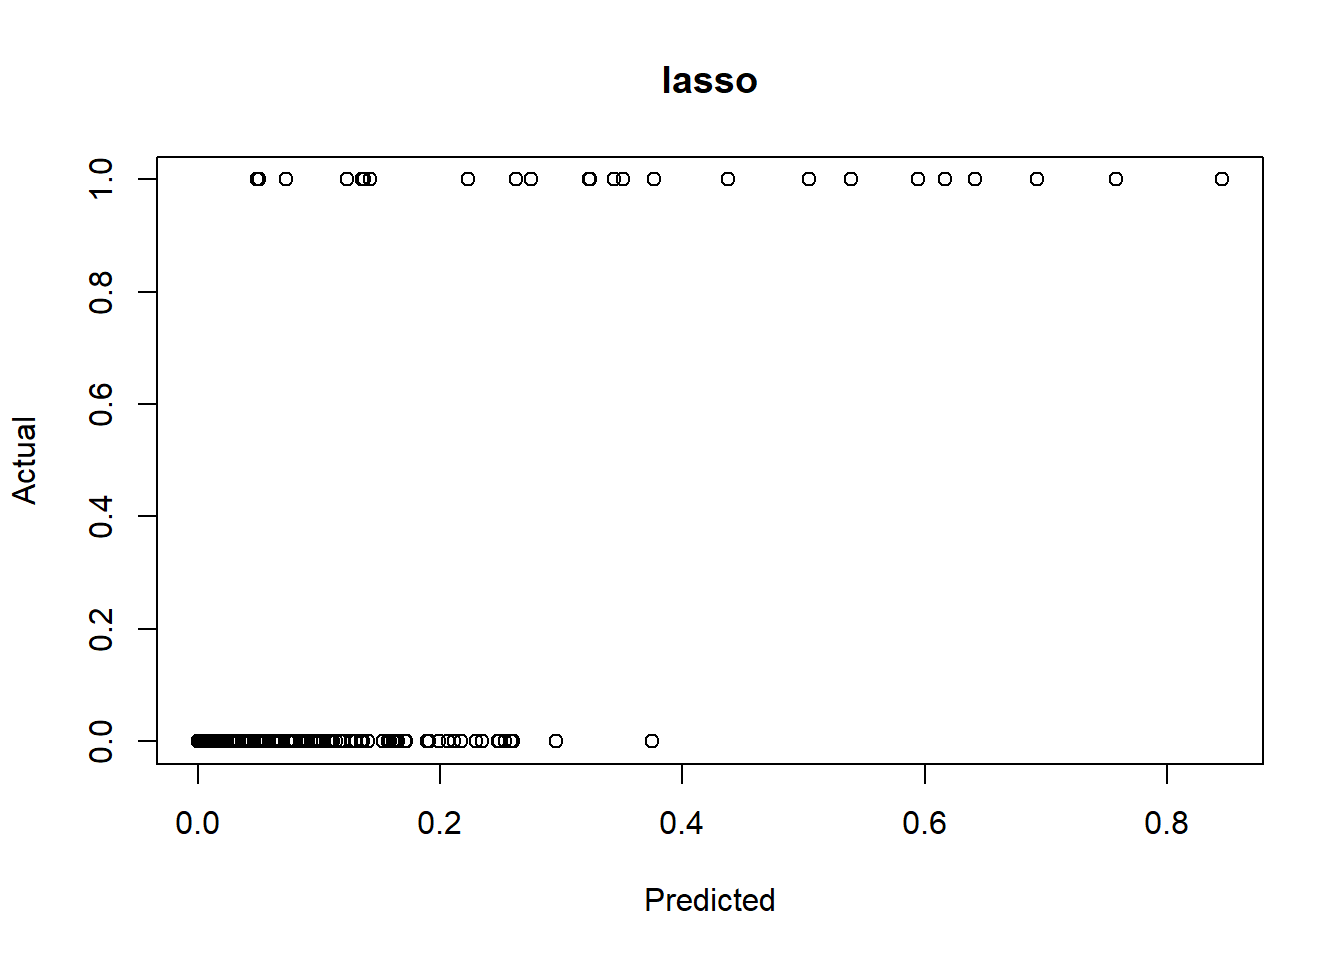
\includegraphics{04-lasso_files/figure-latex/unnamed-chunk-13-1.pdf}

\hypertarget{ux5efaux7acbux6a21ux578bux5e76ux7ed8ux5236ux5217ux7ebfux56fe}{%
\section{建立模型并绘制列线图}\label{ux5efaux7acbux6a21ux578bux5e76ux7ed8ux5236ux5217ux7ebfux56fe}}

\hypertarget{ux5efaux7acbux4e00ux4e2aux6a21ux578bux5427}{%
\subsection{建立一个模型吧}\label{ux5efaux7acbux4e00ux4e2aux6a21ux578bux5427}}

\begin{Shaded}
\begin{Highlighting}[]
\FunctionTok{library}\NormalTok{(rms)}
\end{Highlighting}
\end{Shaded}

\begin{verbatim}
## 载入需要的程辑包:Hmisc
\end{verbatim}

\begin{verbatim}
## 载入需要的程辑包:survival
\end{verbatim}

\begin{verbatim}
## 
## 载入程辑包:'survival'
\end{verbatim}

\begin{verbatim}
## The following object is masked from 'package:caret':
## 
##     cluster
\end{verbatim}

\begin{verbatim}
## 载入需要的程辑包:Formula
\end{verbatim}

\begin{verbatim}
## 
## 载入程辑包:'Hmisc'
\end{verbatim}

\begin{verbatim}
## The following objects are masked from 'package:dplyr':
## 
##     src, summarize
\end{verbatim}

\begin{verbatim}
## The following objects are masked from 'package:base':
## 
##     format.pval, units
\end{verbatim}

\begin{verbatim}
## 载入需要的程辑包:SparseM
\end{verbatim}

\begin{verbatim}
## 
## 载入程辑包:'SparseM'
\end{verbatim}

\begin{verbatim}
## The following object is masked from 'package:base':
## 
##     backsolve
\end{verbatim}

\begin{verbatim}
## 
## 载入程辑包:'rms'
\end{verbatim}

\begin{verbatim}
## The following objects are masked from 'package:car':
## 
##     Predict, vif
\end{verbatim}

\begin{Shaded}
\begin{Highlighting}[]
\NormalTok{dd }\OtherTok{\textless{}{-}} \FunctionTok{datadist}\NormalTok{(myopia)}
\FunctionTok{options}\NormalTok{(}\AttributeTok{datadist=}\NormalTok{dd)}
\NormalTok{model}\OtherTok{\textless{}{-}} \FunctionTok{lrm}\NormalTok{(MYOPIC}\SpecialCharTok{\textasciitilde{}}\NormalTok{SPHEQ}\SpecialCharTok{+}\NormalTok{PARENTS}\SpecialCharTok{+}\NormalTok{GENDER}\SpecialCharTok{+}\NormalTok{ACD}\SpecialCharTok{+}\NormalTok{SPORTHR}\SpecialCharTok{+}\NormalTok{READHR,}\AttributeTok{data=}\NormalTok{myopia,}\AttributeTok{x=}\ConstantTok{TRUE}\NormalTok{,}\AttributeTok{y=}\ConstantTok{TRUE}\NormalTok{)}
\end{Highlighting}
\end{Shaded}

\hypertarget{ux5217ux7ebfux56fe1}{%
\subsection{列线图1}\label{ux5217ux7ebfux56fe1}}

\begin{Shaded}
\begin{Highlighting}[]
\NormalTok{nom1 }\OtherTok{\textless{}{-}} \FunctionTok{nomogram}\NormalTok{(model,}\AttributeTok{fun =}\NormalTok{ plogis,}\AttributeTok{fun.at=}\FunctionTok{c}\NormalTok{(}\FloatTok{0.001}\NormalTok{,}\FloatTok{0.01}\NormalTok{,}\FloatTok{0.05}\NormalTok{,}\FloatTok{0.1}\NormalTok{,}\FunctionTok{seq}\NormalTok{(}\FloatTok{0.2}\NormalTok{,}\FloatTok{0.8}\NormalTok{,}\AttributeTok{by=}\FloatTok{0.2}\NormalTok{),}\FloatTok{0.95}\NormalTok{,}\FloatTok{1.0}\NormalTok{),}\AttributeTok{lp=}\ConstantTok{FALSE}\NormalTok{,}\AttributeTok{funlabel =} \StringTok{\textquotesingle{}myopia\textquotesingle{}}\NormalTok{)}
\FunctionTok{plot}\NormalTok{(nom1)}
\end{Highlighting}
\end{Shaded}

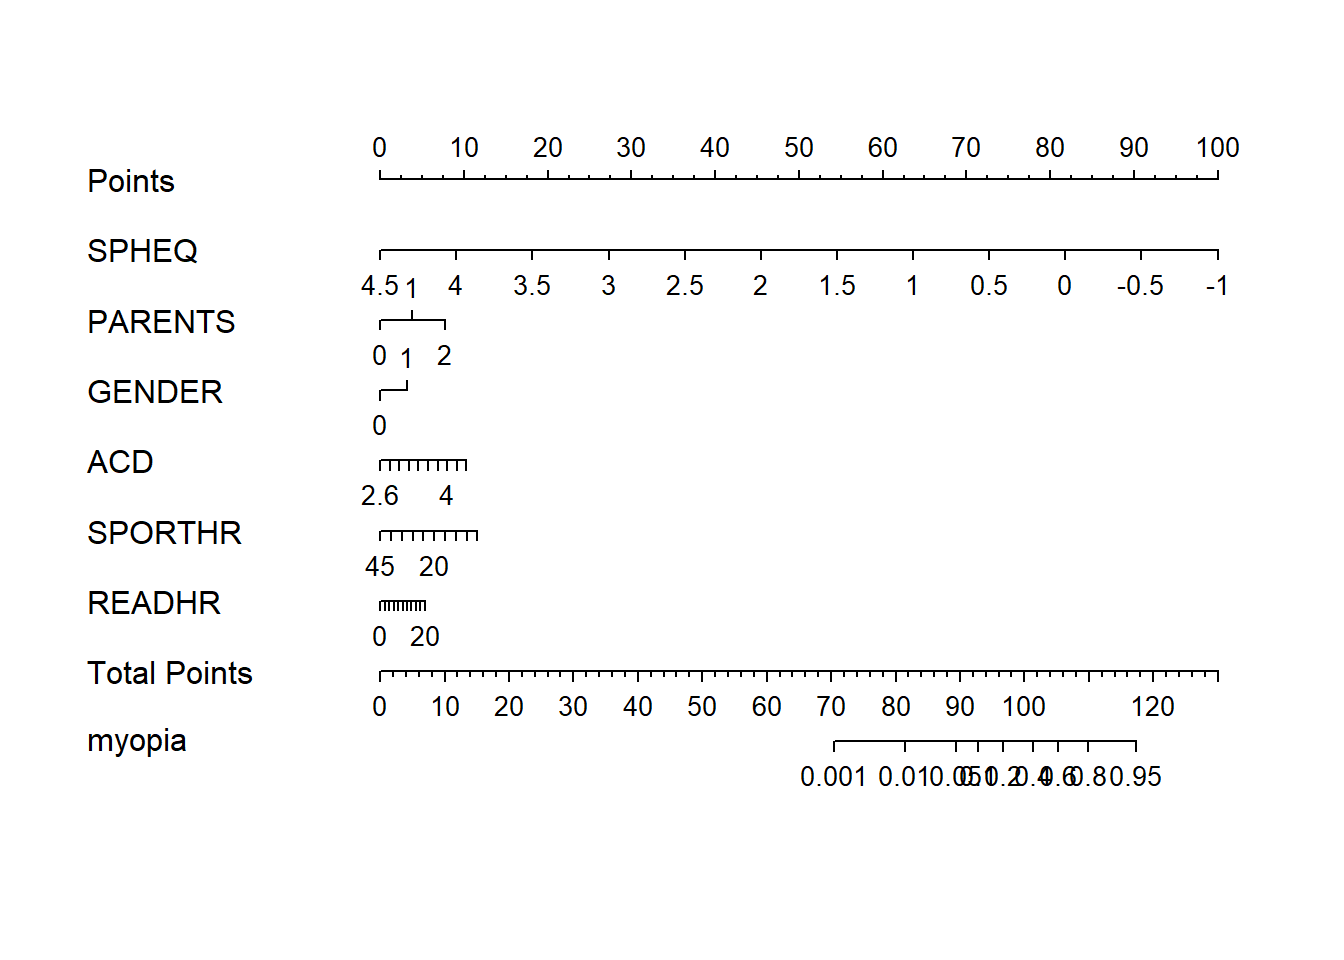
\includegraphics{04-lasso_files/figure-latex/unnamed-chunk-15-1.pdf}
\#\#\# 列线图2

\begin{Shaded}
\begin{Highlighting}[]
\CommentTok{\# \# install.packages("DynNom")}
\CommentTok{\# library(DynNom)}
\CommentTok{\# model\_dynnom \textless{}{-} glm(MYOPIC\textasciitilde{}SPHEQ+PARENTS+GENDER+ACD+SPORTHR+READHR,data=myopia,family = binomial())}
\CommentTok{\# DynNom(model\_dynnom,DNtitle = "Nomogram",DNxlab = "Probability")}
\end{Highlighting}
\end{Shaded}

\hypertarget{cux7edfux8ba1ux91cf}{%
\subsection{C统计量}\label{cux7edfux8ba1ux91cf}}

\begin{Shaded}
\begin{Highlighting}[]
\NormalTok{myopia}\SpecialCharTok{$}\NormalTok{predvalue }\OtherTok{\textless{}{-}} \FunctionTok{predict}\NormalTok{(model)}
\CommentTok{\# install.package(\textquotesingle{}ROCR\textquotesingle{})}
\FunctionTok{library}\NormalTok{(ROCR)}
\end{Highlighting}
\end{Shaded}

\begin{verbatim}
## Warning: 程辑包'ROCR'是用R版本4.1.3 来建造的
\end{verbatim}

\begin{Shaded}
\begin{Highlighting}[]
\NormalTok{pred }\OtherTok{\textless{}{-}} \FunctionTok{prediction}\NormalTok{(myopia}\SpecialCharTok{$}\NormalTok{predvalue,myopia}\SpecialCharTok{$}\NormalTok{MYOPIC)}
\NormalTok{perf }\OtherTok{\textless{}{-}} \FunctionTok{performance}\NormalTok{(pred,}\StringTok{"tpr"}\NormalTok{,}\StringTok{"fpr"}\NormalTok{)}
\FunctionTok{plot}\NormalTok{(perf)}
\FunctionTok{abline}\NormalTok{(}\DecValTok{0}\NormalTok{,}\DecValTok{1}\NormalTok{)}
\end{Highlighting}
\end{Shaded}

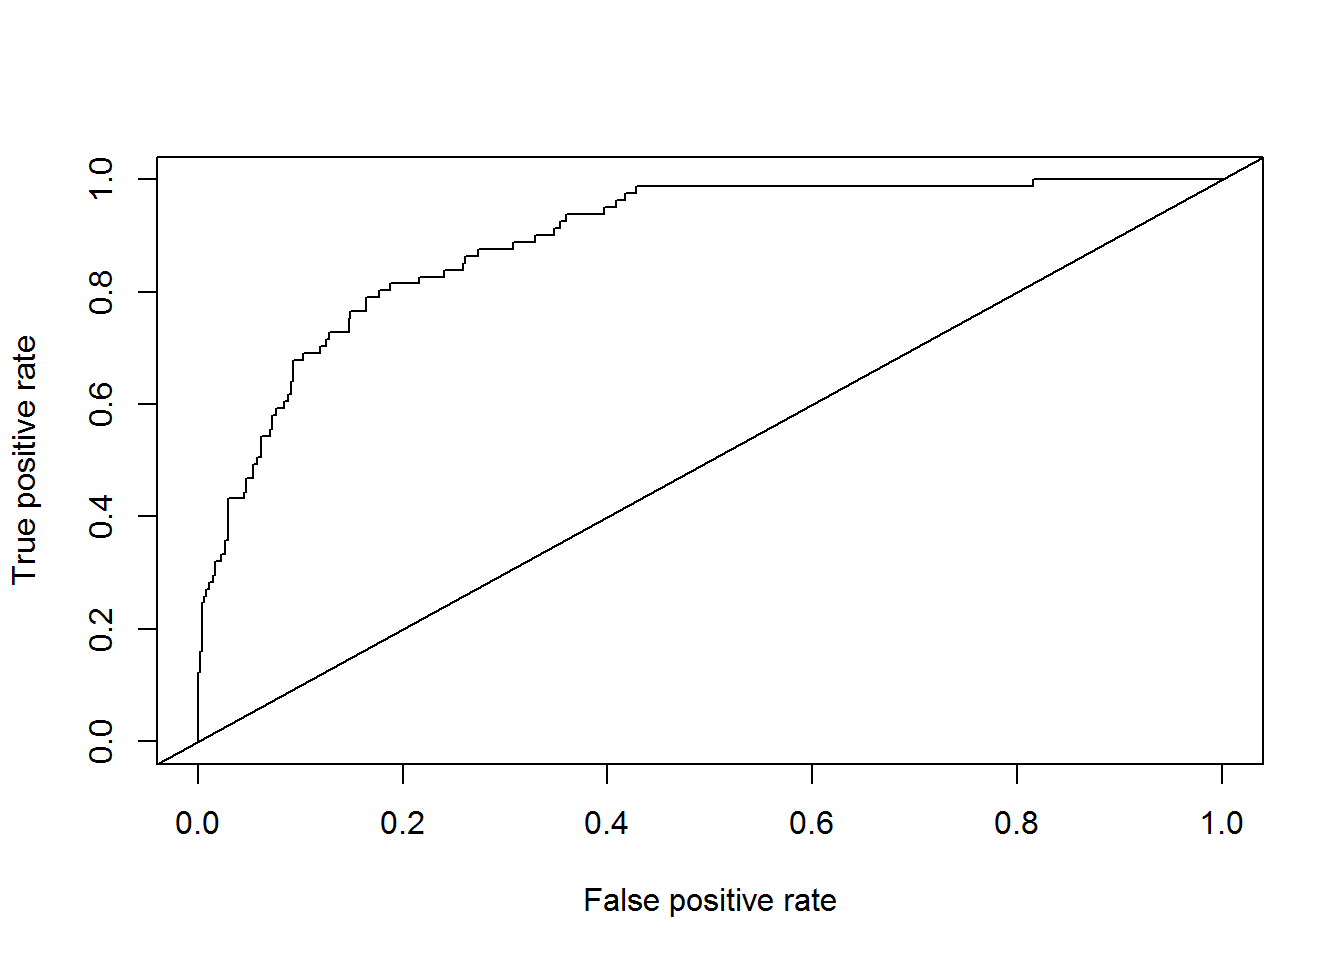
\includegraphics{04-lasso_files/figure-latex/unnamed-chunk-17-1.pdf}

\begin{Shaded}
\begin{Highlighting}[]
\NormalTok{auc }\OtherTok{\textless{}{-}} \FunctionTok{performance}\NormalTok{(pred,}\StringTok{"auc"}\NormalTok{)}
\NormalTok{auc}\SpecialCharTok{@}\NormalTok{y.values}
\end{Highlighting}
\end{Shaded}

\begin{verbatim}
## [[1]]
## [1] 0.8914178
\end{verbatim}

\begin{Shaded}
\begin{Highlighting}[]
\CommentTok{\# model\_glm \textless{}{-} glm(MYOPIC\textasciitilde{}SPHEQ+PARENTS+GENDER+ACD+SPORTHR+READHR,data = myopia,family = binomial())}
\CommentTok{\# myopia$predvalue \textless{}{-} predict(model\_glm)}
\CommentTok{\# \# install.package(\textquotesingle{}ROCR\textquotesingle{})}
\CommentTok{\# library(ROCR)}
\CommentTok{\# pred \textless{}{-} prediction(myopia$predvalue,myopia$MYOPIC)}
\CommentTok{\# perf \textless{}{-} performance(pred,"tpr","fpr")}
\CommentTok{\# plot(perf)}
\CommentTok{\# abline(0,1)}
\CommentTok{\# auc \textless{}{-} performance(pred,"auc")}
\CommentTok{\# auc@y.values}
\end{Highlighting}
\end{Shaded}

\hypertarget{ux6821ux6b63ux66f2ux7ebf}{%
\subsection{校正曲线}\label{ux6821ux6b63ux66f2ux7ebf}}

\begin{Shaded}
\begin{Highlighting}[]
\NormalTok{cal1 }\OtherTok{\textless{}{-}} \FunctionTok{calibrate}\NormalTok{(model,}\AttributeTok{method =} \StringTok{"boot"}\NormalTok{,}\AttributeTok{B=}\DecValTok{1000}\NormalTok{)}
\FunctionTok{plot}\NormalTok{(cal1,}\AttributeTok{xlim=}\FunctionTok{c}\NormalTok{(}\DecValTok{0}\NormalTok{,}\FloatTok{1.0}\NormalTok{),}\AttributeTok{ylim=}\FunctionTok{c}\NormalTok{(}\DecValTok{0}\NormalTok{,}\FloatTok{1.0}\NormalTok{))}
\end{Highlighting}
\end{Shaded}

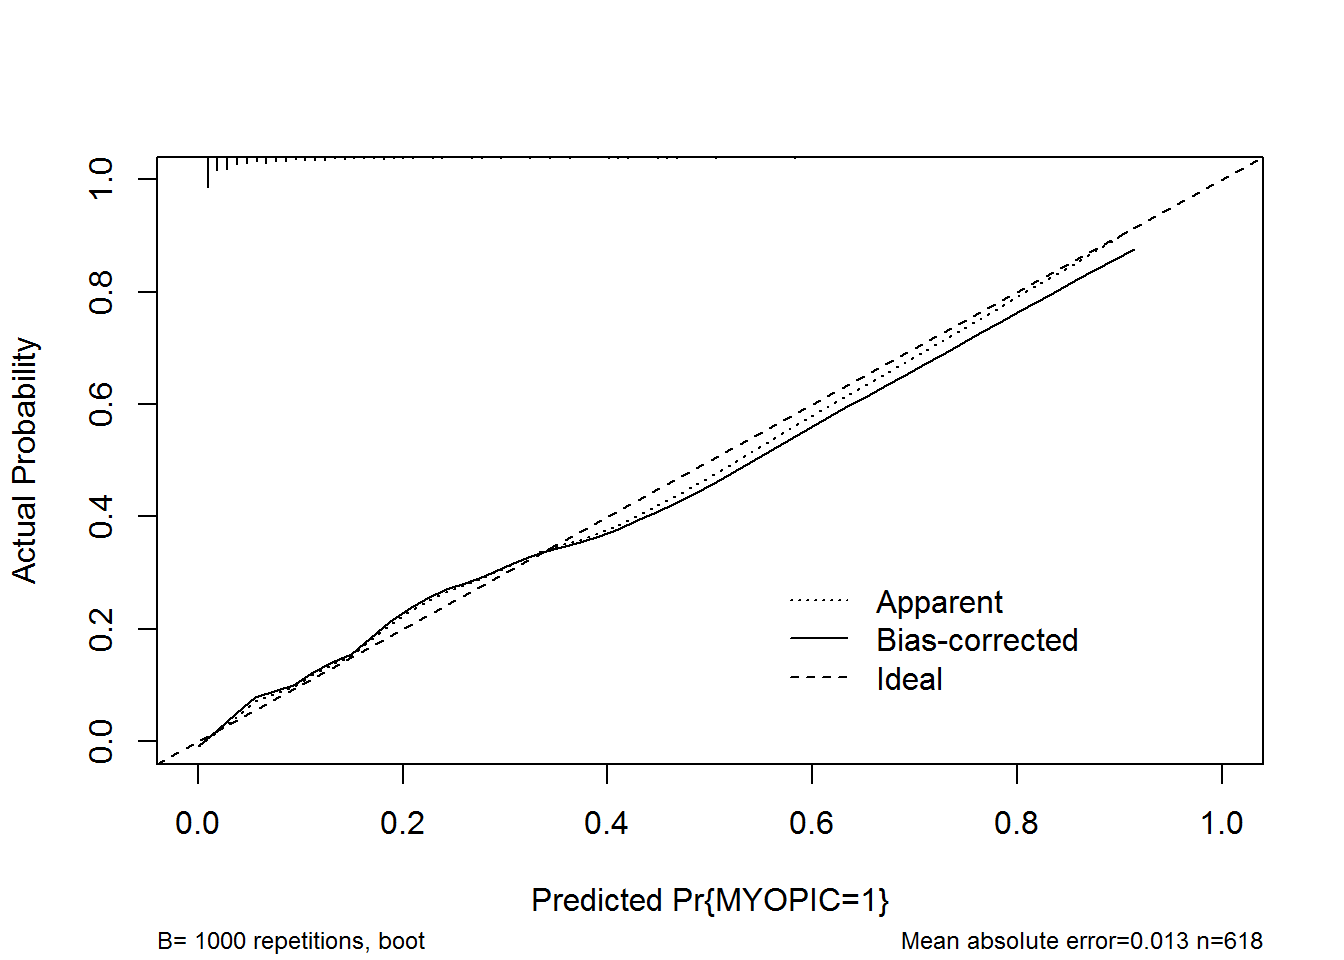
\includegraphics{04-lasso_files/figure-latex/unnamed-chunk-19-1.pdf}

\begin{verbatim}
## 
## n=618   Mean absolute error=0.013   Mean squared error=3e-04
## 0.9 Quantile of absolute error=0.032
\end{verbatim}

\hypertarget{psux540cux65f6ux7ed8ux5236ux591aux6761}{%
\subsection{ps:同时绘制多条}\label{psux540cux65f6ux7ed8ux5236ux591aux6761}}

\begin{Shaded}
\begin{Highlighting}[]
\NormalTok{formula1 }\OtherTok{\textless{}{-}} \FunctionTok{as.formula}\NormalTok{(MYOPIC}\SpecialCharTok{\textasciitilde{}}\NormalTok{SPHEQ)}

\NormalTok{formula2 }\OtherTok{\textless{}{-}} \FunctionTok{as.formula}\NormalTok{(MYOPIC}\SpecialCharTok{\textasciitilde{}}\NormalTok{SPHEQ}\SpecialCharTok{+}\NormalTok{PARENTS}\SpecialCharTok{+}\NormalTok{GENDER}\SpecialCharTok{+}\NormalTok{ACD}\SpecialCharTok{+}\NormalTok{SPORTHR}\SpecialCharTok{+}\NormalTok{READHR)}

\NormalTok{formula3 }\OtherTok{\textless{}{-}} \FunctionTok{as.formula}\NormalTok{(MYOPIC}\SpecialCharTok{\textasciitilde{}}\NormalTok{PARENTS}\SpecialCharTok{+}\NormalTok{GENDER}\SpecialCharTok{+}\NormalTok{ACD}\SpecialCharTok{+}\NormalTok{SPORTHR}\SpecialCharTok{+}\NormalTok{READHR)}

\NormalTok{DD}\OtherTok{=}\FunctionTok{datadist}\NormalTok{(myopia)}
\FunctionTok{options}\NormalTok{(}\AttributeTok{datadist=}\StringTok{\textquotesingle{}DD\textquotesingle{}}\NormalTok{)}
\end{Highlighting}
\end{Shaded}

\begin{Shaded}
\begin{Highlighting}[]
\NormalTok{fit1 }\OtherTok{=} \FunctionTok{glm}\NormalTok{(formula1, }\AttributeTok{data=}\NormalTok{myopia,}\AttributeTok{family =} \FunctionTok{binomial}\NormalTok{())}
\NormalTok{fit2 }\OtherTok{=} \FunctionTok{glm}\NormalTok{(formula2, }\AttributeTok{data=}\NormalTok{myopia,}\AttributeTok{family =} \FunctionTok{binomial}\NormalTok{())}
\NormalTok{fit3 }\OtherTok{=} \FunctionTok{glm}\NormalTok{(formula3, }\AttributeTok{data=}\NormalTok{myopia,}\AttributeTok{family =} \FunctionTok{binomial}\NormalTok{())}


\FunctionTok{library}\NormalTok{(riskRegression)}
\end{Highlighting}
\end{Shaded}

\begin{verbatim}
## Warning: 程辑包'riskRegression'是用R版本4.1.3 来建造的
\end{verbatim}

\begin{verbatim}
## riskRegression version 2022.03.22
\end{verbatim}

\begin{Shaded}
\begin{Highlighting}[]
\NormalTok{xb }\OtherTok{\textless{}{-}} \FunctionTok{Score}\NormalTok{(}\FunctionTok{list}\NormalTok{(}\StringTok{"fit1"}\OtherTok{=}\NormalTok{fit1,}
                 \StringTok{"fit2"}\OtherTok{=}\NormalTok{fit2,}
                 \StringTok{"fit3"}\OtherTok{=}\NormalTok{fit3),}
            \AttributeTok{formula=}\NormalTok{MYOPIC}\SpecialCharTok{\textasciitilde{}}\DecValTok{1}\NormalTok{,}
            \AttributeTok{null.model =} \ConstantTok{FALSE}\NormalTok{,}
            \AttributeTok{conf.int =}\ConstantTok{TRUE}\NormalTok{,}
            \AttributeTok{plots =}\FunctionTok{c}\NormalTok{(}\StringTok{"calibration"}\NormalTok{,}\StringTok{"ROC"}\NormalTok{),}
            \AttributeTok{metrics =} \FunctionTok{c}\NormalTok{(}\StringTok{"auc"}\NormalTok{),}
            \AttributeTok{B=}\DecValTok{1000}\NormalTok{,}\AttributeTok{M=}\DecValTok{50}\NormalTok{,}
            \AttributeTok{data=}\NormalTok{myopia)}
\FunctionTok{plotCalibration}\NormalTok{(xb)}
\end{Highlighting}
\end{Shaded}

\begin{verbatim}
## Warning in getLegendData(object = x, models = models, times = tp, auc.in.legend
## = auc.in.legend, : Cannot show Brier score as it is not stored in object. Set
## metrics='brier' in the call of Score.
\end{verbatim}

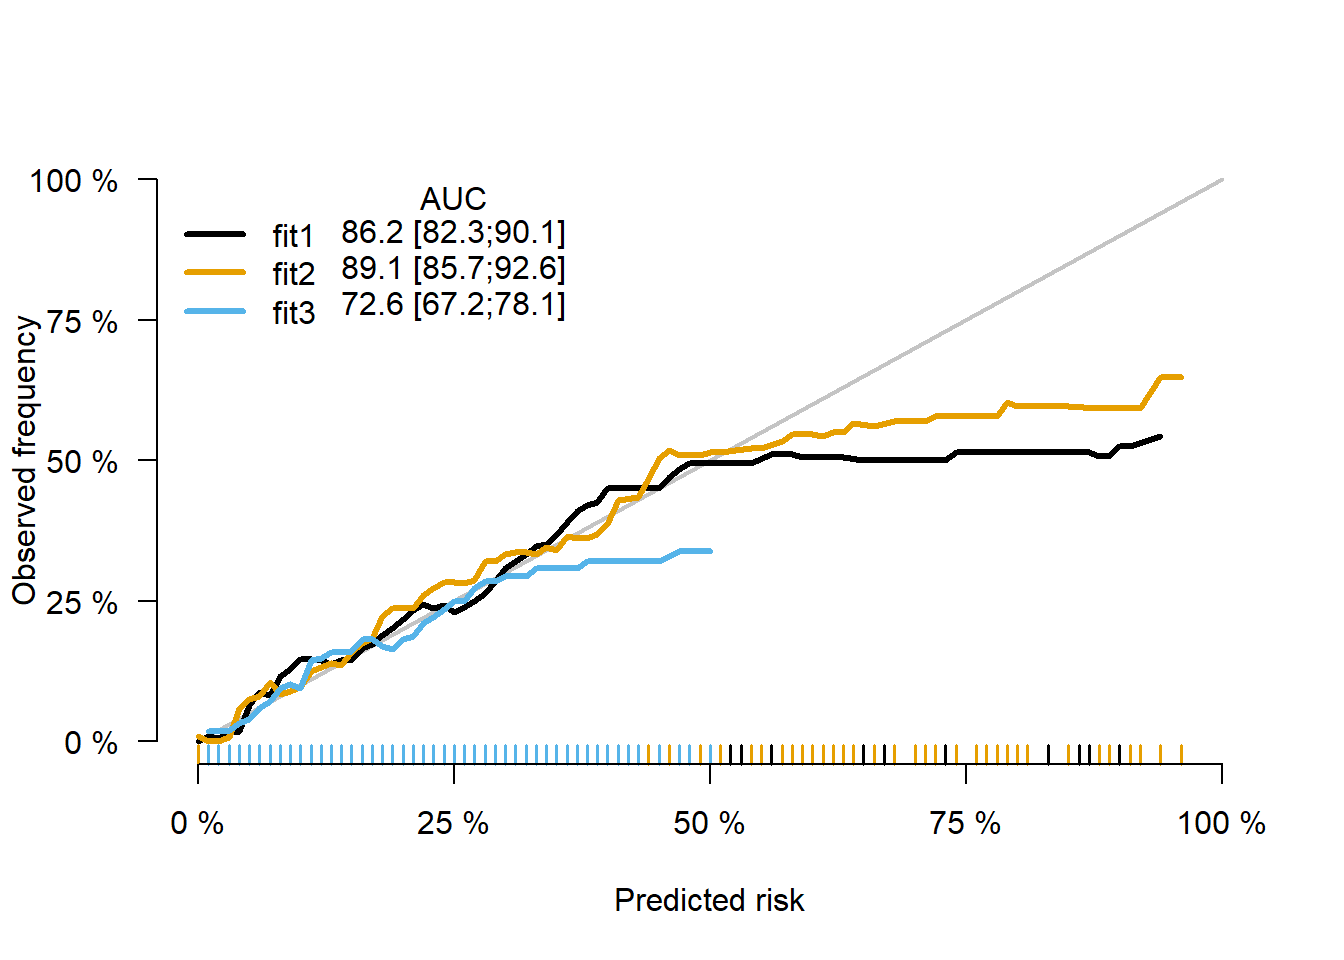
\includegraphics{04-lasso_files/figure-latex/unnamed-chunk-21-1.pdf}

\hypertarget{ux5171ux7ebfux6027ux8ba8ux8bba}{%
\section{共线性讨论}\label{ux5171ux7ebfux6027ux8ba8ux8bba}}

\begin{Shaded}
\begin{Highlighting}[]
\CommentTok{\#collinearity }
\NormalTok{collin }\OtherTok{\textless{}{-}} \FunctionTok{cor}\NormalTok{(}\FunctionTok{subset}\NormalTok{(myopia, }\AttributeTok{select=}\FunctionTok{c}\NormalTok{(SPHEQ, PARENTS, SPORTHR, GENDER ,ACD , STUDYHR,READHR)))}
\CommentTok{\# dev.off()}
\FunctionTok{library}\NormalTok{(corrplot)}
\FunctionTok{corrplot}\NormalTok{(collin , }\AttributeTok{type=}\StringTok{"upper"}\NormalTok{)}
\end{Highlighting}
\end{Shaded}

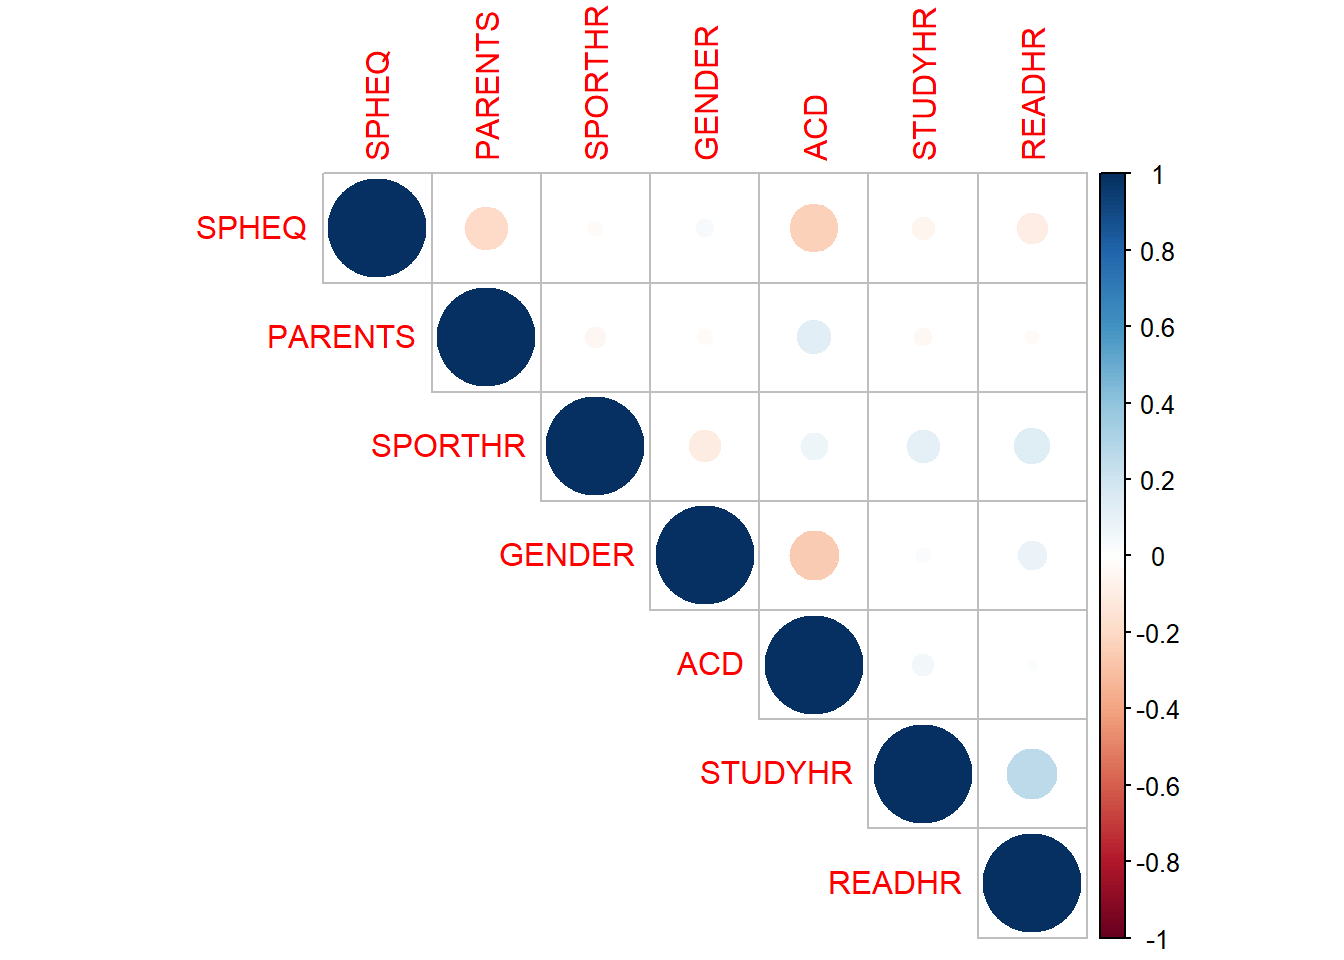
\includegraphics{04-lasso_files/figure-latex/unnamed-chunk-22-1.pdf}

\begin{Shaded}
\begin{Highlighting}[]
\NormalTok{M }\OtherTok{\textless{}{-}}\NormalTok{ collin}
\NormalTok{cor.mtest }\OtherTok{\textless{}{-}} \ControlFlowTok{function}\NormalTok{(mat, ...) \{}
\NormalTok{  mat }\OtherTok{\textless{}{-}} \FunctionTok{as.matrix}\NormalTok{(mat)}
\NormalTok{  n }\OtherTok{\textless{}{-}} \FunctionTok{ncol}\NormalTok{(mat)}
\NormalTok{  p.mat}\OtherTok{\textless{}{-}} \FunctionTok{matrix}\NormalTok{(}\ConstantTok{NA}\NormalTok{, n, n)}
  \FunctionTok{diag}\NormalTok{(p.mat) }\OtherTok{\textless{}{-}} \DecValTok{0}
  \ControlFlowTok{for}\NormalTok{ (i }\ControlFlowTok{in} \DecValTok{1}\SpecialCharTok{:}\NormalTok{(n }\SpecialCharTok{{-}} \DecValTok{1}\NormalTok{)) \{}
    \ControlFlowTok{for}\NormalTok{ (j }\ControlFlowTok{in}\NormalTok{ (i }\SpecialCharTok{+} \DecValTok{1}\NormalTok{)}\SpecialCharTok{:}\NormalTok{n) \{}
\NormalTok{      tmp }\OtherTok{\textless{}{-}} \FunctionTok{cor.test}\NormalTok{(mat[, i], mat[, j], ...)}
\NormalTok{      p.mat[i, j] }\OtherTok{\textless{}{-}}\NormalTok{ p.mat[j, i] }\OtherTok{\textless{}{-}}\NormalTok{ tmp}\SpecialCharTok{$}\NormalTok{p.value}
\NormalTok{    \}}
\NormalTok{  \}}
  \FunctionTok{colnames}\NormalTok{(p.mat) }\OtherTok{\textless{}{-}} \FunctionTok{rownames}\NormalTok{(p.mat) }\OtherTok{\textless{}{-}} \FunctionTok{colnames}\NormalTok{(mat)}
\NormalTok{  p.mat}
\NormalTok{\}}
\CommentTok{\# matrix of the p{-}value of the correlation}
\NormalTok{p.mat }\OtherTok{\textless{}{-}} \FunctionTok{cor.mtest}\NormalTok{(}\FunctionTok{subset}\NormalTok{(myopia, }\AttributeTok{select=}\FunctionTok{c}\NormalTok{(SPHEQ, PARENTS,  }
\NormalTok{                                           SPORTHR, GENDER ,ACD , STUDYHR,READHR)))}
\FunctionTok{head}\NormalTok{(p.mat[, }\DecValTok{1}\SpecialCharTok{:}\DecValTok{6}\NormalTok{])}
\end{Highlighting}
\end{Shaded}

\begin{verbatim}
##                SPHEQ      PARENTS     SPORTHR       GENDER          ACD
## SPHEQ   0.000000e+00 1.351303e-06 0.577189469 4.206886e-01 1.841368e-09
## PARENTS 1.351303e-06 0.000000e+00 0.270789297 5.333279e-01 2.718984e-03
## SPORTHR 5.771895e-01 2.707893e-01 0.000000000 1.025312e-02 6.185484e-02
## GENDER  4.206886e-01 5.333279e-01 0.010253119 0.000000e+00 1.757790e-10
## ACD     1.841368e-09 2.718984e-03 0.061854843 1.757790e-10 0.000000e+00
## STUDYHR 1.730743e-01 3.891322e-01 0.003930083 5.391071e-01 1.982234e-01
##             STUDYHR
## SPHEQ   0.173074294
## PARENTS 0.389132155
## SPORTHR 0.003930083
## GENDER  0.539107149
## ACD     0.198223365
## STUDYHR 0.000000000
\end{verbatim}

\begin{Shaded}
\begin{Highlighting}[]
\NormalTok{col }\OtherTok{\textless{}{-}} \FunctionTok{colorRampPalette}\NormalTok{(}\FunctionTok{c}\NormalTok{(}\StringTok{"\#BB4444"}\NormalTok{, }\StringTok{"\#EE9988"}\NormalTok{, }\StringTok{"\#FFFFFF"}\NormalTok{, }
                          \StringTok{"\#77AADD"}\NormalTok{, }\StringTok{"\#4477AA"}\NormalTok{))}

\CommentTok{\#create correlation plot}
\FunctionTok{corrplot}\NormalTok{(M, }\AttributeTok{method=}\StringTok{"color"}\NormalTok{, }\AttributeTok{col=}\FunctionTok{col}\NormalTok{(}\DecValTok{200}\NormalTok{),  }
         \AttributeTok{type=}\StringTok{"upper"}\NormalTok{, }\AttributeTok{order=}\StringTok{"hclust"}\NormalTok{, }
         \AttributeTok{addCoef.col =} \StringTok{"black"}\NormalTok{, }\CommentTok{\# Add coefficient of correlation}
         \AttributeTok{tl.col=}\StringTok{"black"}\NormalTok{, }\AttributeTok{tl.srt=}\DecValTok{45}\NormalTok{, }\CommentTok{\#Text label color and rotation}
         \CommentTok{\# Combine with significance}
         \AttributeTok{p.mat =}\NormalTok{ p.mat, }\AttributeTok{sig.level =} \FloatTok{0.01}\NormalTok{, }\AttributeTok{insig =} \StringTok{"blank"}\NormalTok{, }
         \CommentTok{\# hide correlation coefficient on the principal diagonal}
         \AttributeTok{diag=}\ConstantTok{FALSE}\NormalTok{ )}
\end{Highlighting}
\end{Shaded}

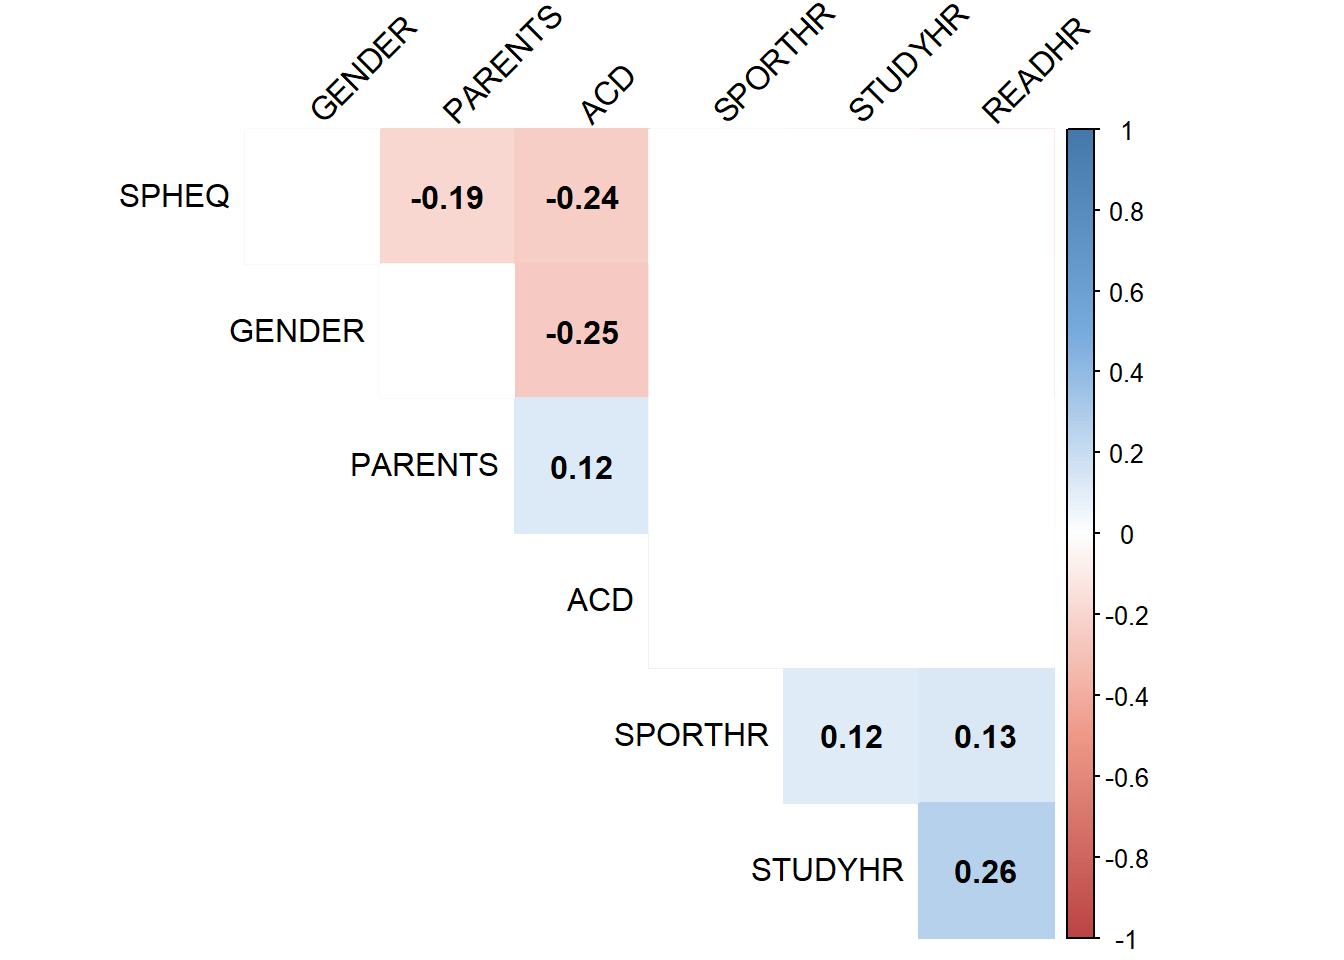
\includegraphics{04-lasso_files/figure-latex/unnamed-chunk-22-2.pdf}

\begin{Shaded}
\begin{Highlighting}[]
\FunctionTok{vif}\NormalTok{(model)}
\end{Highlighting}
\end{Shaded}

\begin{verbatim}
##    SPHEQ  PARENTS   GENDER      ACD  SPORTHR   READHR 
## 1.034080 1.032454 1.101447 1.092771 1.054899 1.060157
\end{verbatim}

VIF 值 \textgreater= 10 表示高共线性。在这种情况下,所有 vif 值都接近 小于10

\cleardoublepage

\hypertarget{appendix-ux9644ux5f55}{%
\appendix \addcontentsline{toc}{chapter}{\appendixname}}


\hypertarget{sound}{%
\chapter{余音绕梁}\label{sound}}

呐,到这里朕的书差不多写完了,但还有几句话要交待,所以开个附录,再啰嗦几句,各位客官稍安勿躁、扶稳坐好。

\bibliography{book.bib,packages.bib}

\backmatter
\printindex

\end{document}
